\documentclass[]{article}
\usepackage{lmodern}
\usepackage{amssymb,amsmath}
\usepackage{ifxetex,ifluatex}
\usepackage{fixltx2e} % provides \textsubscript
\ifnum 0\ifxetex 1\fi\ifluatex 1\fi=0 % if pdftex
  \usepackage[T1]{fontenc}
  \usepackage[utf8]{inputenc}
\else % if luatex or xelatex
  \ifxetex
    \usepackage{mathspec}
  \else
    \usepackage{fontspec}
  \fi
  \defaultfontfeatures{Ligatures=TeX,Scale=MatchLowercase}
\fi
% use upquote if available, for straight quotes in verbatim environments
\IfFileExists{upquote.sty}{\usepackage{upquote}}{}
% use microtype if available
\IfFileExists{microtype.sty}{%
\usepackage{microtype}
\UseMicrotypeSet[protrusion]{basicmath} % disable protrusion for tt fonts
}{}
\usepackage[margin=1in]{geometry}
\usepackage{hyperref}
\hypersetup{unicode=true,
            pdftitle={Analysis of Software and Data Carpentry's Pre- and Post-Workshop Surveys},
            pdfborder={0 0 0},
            breaklinks=true}
\urlstyle{same}  % don't use monospace font for urls
\usepackage{longtable,booktabs}
\usepackage{graphicx,grffile}
\makeatletter
\def\maxwidth{\ifdim\Gin@nat@width>\linewidth\linewidth\else\Gin@nat@width\fi}
\def\maxheight{\ifdim\Gin@nat@height>\textheight\textheight\else\Gin@nat@height\fi}
\makeatother
% Scale images if necessary, so that they will not overflow the page
% margins by default, and it is still possible to overwrite the defaults
% using explicit options in \includegraphics[width, height, ...]{}
\setkeys{Gin}{width=\maxwidth,height=\maxheight,keepaspectratio}
\IfFileExists{parskip.sty}{%
\usepackage{parskip}
}{% else
\setlength{\parindent}{0pt}
\setlength{\parskip}{6pt plus 2pt minus 1pt}
}
\setlength{\emergencystretch}{3em}  % prevent overfull lines
\providecommand{\tightlist}{%
  \setlength{\itemsep}{0pt}\setlength{\parskip}{0pt}}
\setcounter{secnumdepth}{0}
% Redefines (sub)paragraphs to behave more like sections
\ifx\paragraph\undefined\else
\let\oldparagraph\paragraph
\renewcommand{\paragraph}[1]{\oldparagraph{#1}\mbox{}}
\fi
\ifx\subparagraph\undefined\else
\let\oldsubparagraph\subparagraph
\renewcommand{\subparagraph}[1]{\oldsubparagraph{#1}\mbox{}}
\fi

%%% Use protect on footnotes to avoid problems with footnotes in titles
\let\rmarkdownfootnote\footnote%
\def\footnote{\protect\rmarkdownfootnote}

%%% Change title format to be more compact
\usepackage{titling}

% Create subtitle command for use in maketitle
\newcommand{\subtitle}[1]{
  \posttitle{
    \begin{center}\large#1\end{center}
    }
}

\setlength{\droptitle}{-2em}
  \title{Analysis of Software and Data Carpentry's Pre- and Post-Workshop Surveys}
  \pretitle{\vspace{\droptitle}\centering\huge}
  \posttitle{\par}
  \author{}
  \preauthor{}\postauthor{}
  \predate{\centering\large\emph}
  \postdate{\par}
  \date{September 30, 2018}


\begin{document}
\maketitle

{
\setcounter{tocdepth}{2}
\tableofcontents
}
\subsection{Overview}\label{overview}

Since February 12, 2016, Software and Data Carpentry have collected
information on learner demographics, perception of tools, and confidence
in working with data. As a benefit of partnering with the Carpentries,
the Assessment Team will release bi-annual reports of the results of
pre- and post-workshop surveys, customized for each member organization.

This report covers the workshops from February 12, 2016 to May 21, 2018
for Software Carpentry, and from August 07, 2017 to May 11, 2018 for
Data Carpentry.

As an overview, 1490 and 854 learners have responded to Data Carpentry
pre- and post-workshop surveys respectively at your institution, while
1346 and 617 have responded to Software Carpentry workshop surveys.

This report includes the following:

\begin{itemize}
\tightlist
\item
  Motivation for Attending Carpentries Workshops
\item
  Workshop Type and Perception of Workshop Environment/Experience
\item
  Effect of Workshops on Learners' Self-Reported Perspectives, Skills,
  and Confidence
\item
  Ability to Perform Computing Tasks
\item
  Demographics
\item
  Summary
\end{itemize}

\subsection{Motivation for Attending Carpentries
Workshops}\label{motivation-for-attending-carpentries-workshops}

Understanding why learners attend Carpentries workshops may help you in
your strategy to organize and host workshops. Remember, Data Carpentry's
workshops are domain-specific and focus on the fundamental data skills
needed to conduct research. Many Data Carpentry workshops include
lessons on data organization and include data cleaning with OpenRefine.
From there, learners spend time learning a programming language, either
Python or R, to manipulate and visualize data. Additionally, Data
Carpentry workshops may include Cloud Computing and other topics.

\subsubsection{Why are learners participating in your
workshops?}\label{why-are-learners-participating-in-your-workshops}

Respondents were asked to check all that apply for several factors
provided in the tables below.

\begin{longtable}[]{@{}lrr@{}}
\toprule
Why learners attend Data Carpentry workshops? (n = 1245) & n &
\%\tabularnewline
\midrule
\endhead
To learn skills that I can apply to my current work & 1058 &
85.0\tabularnewline
To learn skills that I can apply to my work in the future & 960 &
77.1\tabularnewline
To learn skills that will help me get a job & 445 & 35.7\tabularnewline
As a requirement for my program/current position & 103 &
8.3\tabularnewline
Other & 47 & 3.8\tabularnewline
\bottomrule
\end{longtable}

85\% of Data Carpentry learners attended workshops at your institution
to learn skills they can apply to their current work.

Software Carpentry's curriculum teaches basic lab skills for scientific
computing. These workshops include automation with the Unix shell,
version control with Git, and programming with R or Python. These tools
help learners to increase the efficiency and reproducibility of their
computational work.

\begin{longtable}[]{@{}lrr@{}}
\toprule
Why learners attend Software Carpentry Workshops? (n = 74) & n &
\%\tabularnewline
\midrule
\endhead
To cover new/additional topics & 50 & 67.6\tabularnewline
To refresh/review skills & 36 & 48.6\tabularnewline
To network & 9 & 12.2\tabularnewline
To help host/run a workshop & 6 & 8.1\tabularnewline
To become a Software Carpentry helper/instructor & 6 &
8.1\tabularnewline
Other & 5 & 6.8\tabularnewline
\bottomrule
\end{longtable}

\begin{longtable}[]{@{}lrr@{}}
\toprule
Software Carpentry 1st Time Learners & n & \%\tabularnewline
\midrule
\endhead
Yes & 1050 & 78.0\tabularnewline
Didn't answer & 219 & 16.3\tabularnewline
No & 77 & 5.7\tabularnewline
\bottomrule
\end{longtable}

Compared to Data Carpentry's learners, Software Carpentry's tend to have
more experience with the tools covered in the workshops, and learners
come to learn new and/or additional topics (67.6\%). For the workshops
at your institution, 78\% of Software Carpentry respondents are
first-time attendees.

\subsubsection{What is the current level of satisfaction of the data
management practices of your learners before attending workshops at your
institution?}\label{what-is-the-current-level-of-satisfaction-of-the-data-management-practices-of-your-learners-before-attending-workshops-at-your-institution}

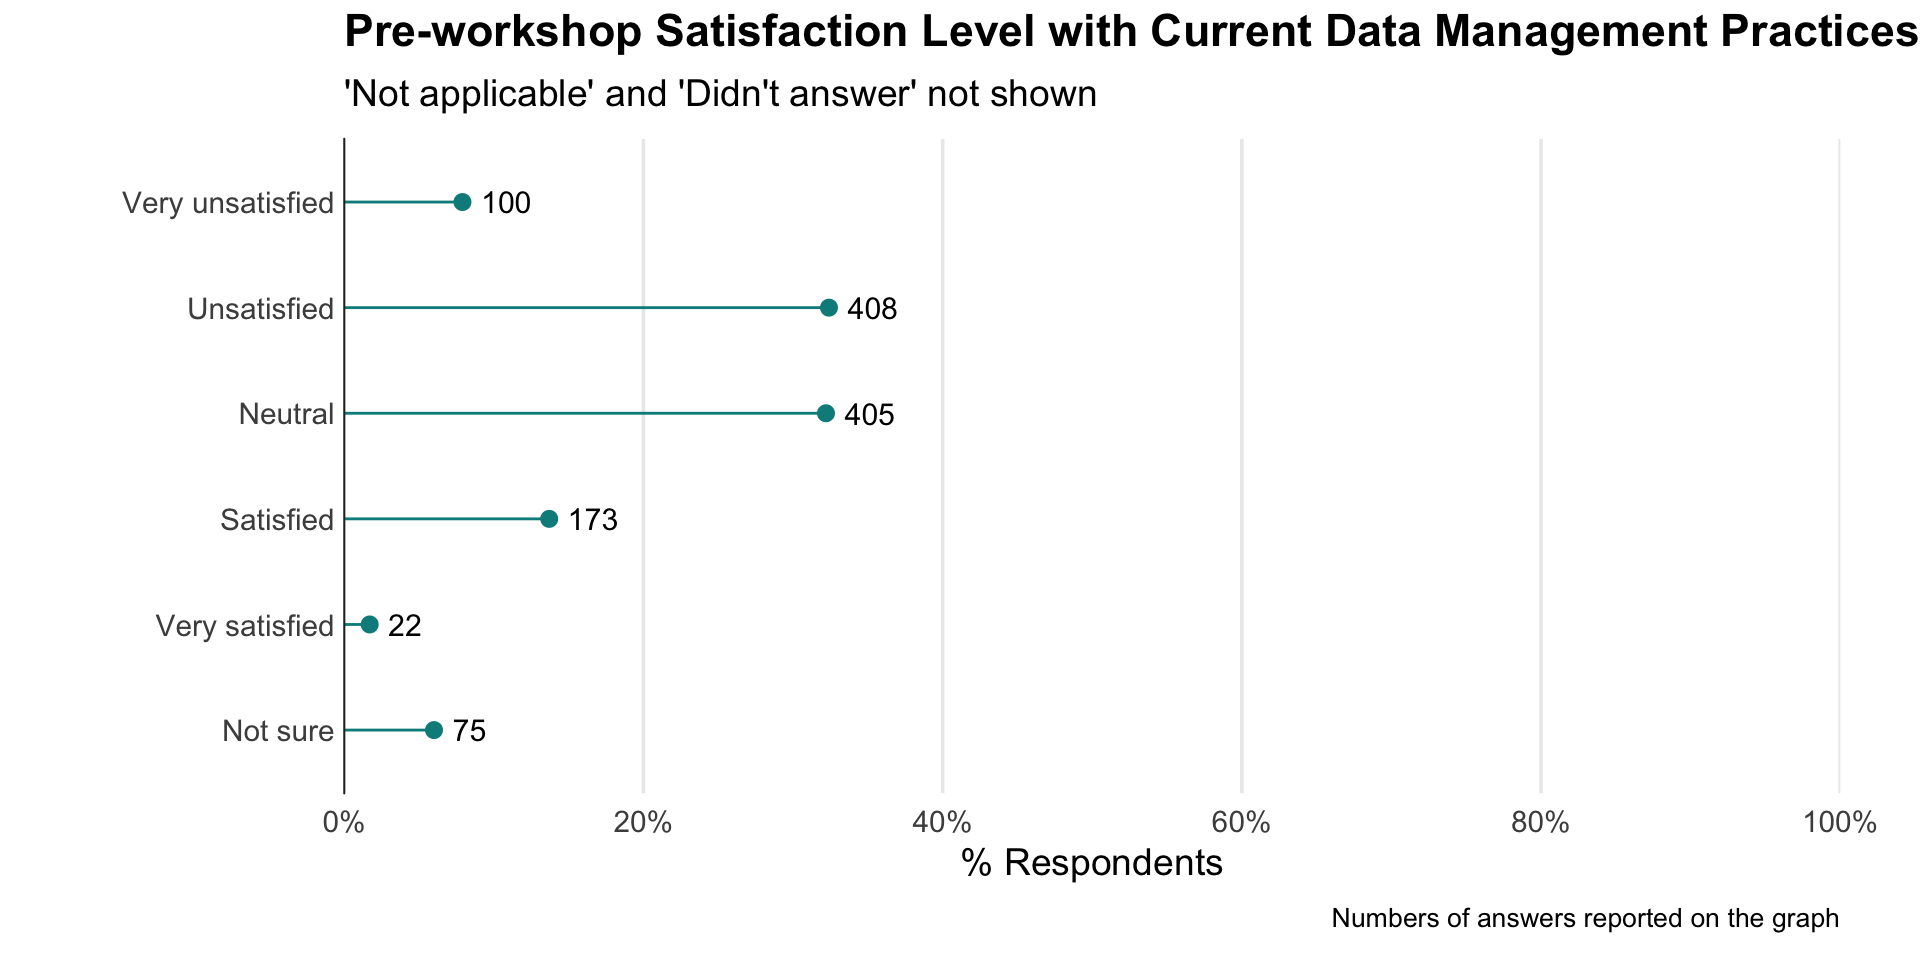
\includegraphics[width=\maxwidth]{../figures/dc-satisfaction-level-plot-1}

The majority (61.3\%) of your Data Carpentry workshop respondents are
either unsatisfied or feel neutral with their current data management
practices. By data management practices, we mean behaviors such as
keeping raw data raw, reusing code, and using databases, queries, and
scripts to manage large data sets.

\subsubsection{How often did your workshop participants program before
attending a workshop at your
institution?}\label{how-often-did-your-workshop-participants-program-before-attending-a-workshop-at-your-institution}

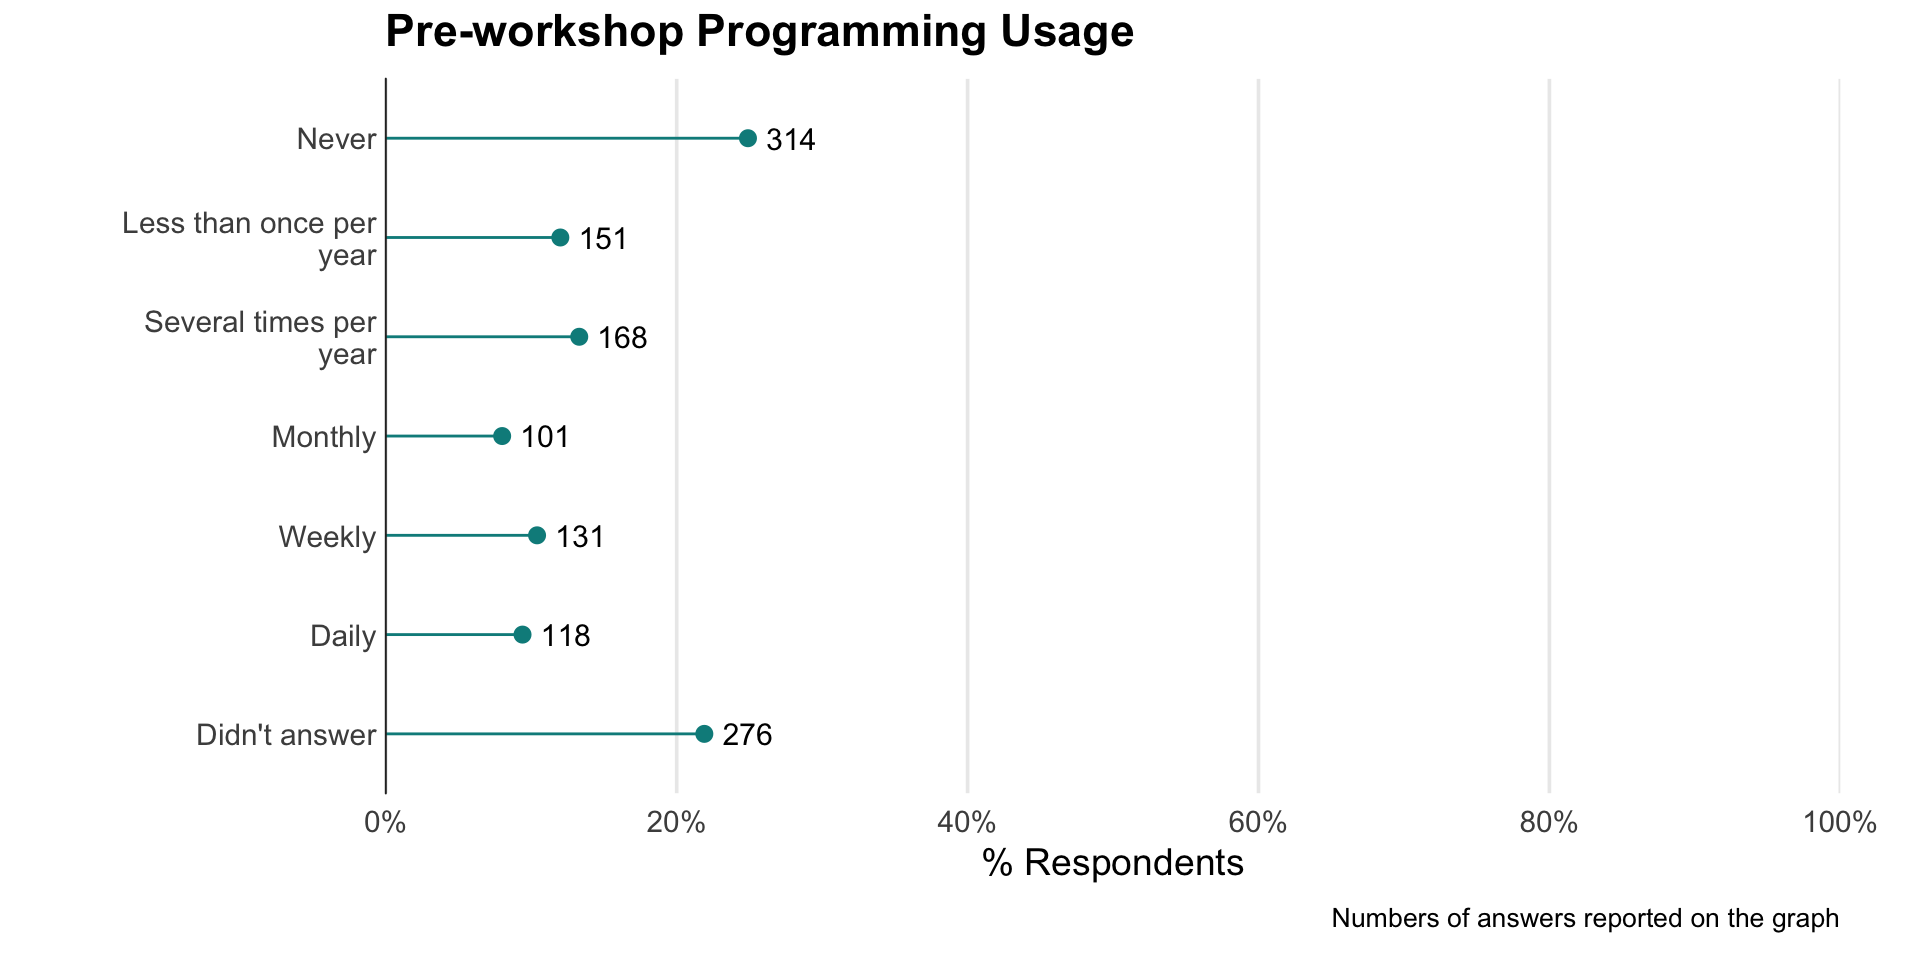
\includegraphics[width=\maxwidth]{../figures/dc-programming-level-plot-1}

In terms of current programming usage, 31.2\% of learners either never
use programming, use programming less than once per year, or no more
than several times per year. Only 7.9\% program on a daily basis.

\begin{longtable}[]{@{}lrr@{}}
\toprule
How respondents find out about Data Carpentry workshops (n =1243) & n &
\%\tabularnewline
\midrule
\endhead
Received an email about the workshop & 802 & 64.5\tabularnewline
My friend/colleague told me about it & 324 & 26.1\tabularnewline
My advisor/supervisor told me about it & 244 & 19.6\tabularnewline
Read about it in a newsletter or university web site & 85 &
6.8\tabularnewline
Other & 49 & 3.9\tabularnewline
Other web site & 20 & 1.6\tabularnewline
Twitter or other social media & 17 & 1.4\tabularnewline
\bottomrule
\end{longtable}

\begin{longtable}[]{@{}lrr@{}}
\toprule
How respondents find out about Software Carpentry workshops (n = 985) &
n & \%\tabularnewline
\midrule
\endhead
Institution mailing list or flyer & 514 & 52.2\tabularnewline
Friend/colleague & 420 & 42.6\tabularnewline
Other & 77 & 7.8\tabularnewline
Conference/meeting/seminar & 42 & 4.3\tabularnewline
Our website & 31 & 3.1\tabularnewline
Funding organization or program officer & 26 & 2.6\tabularnewline
Social Media (Twitter, Facebook, etc.) & 21 & 2.1\tabularnewline
Journal or publication & 3 & 0.3\tabularnewline
\bottomrule
\end{longtable}

Data Carpentry and Software Carpentry workshop participants often found
out about our workshops through institutional mailing lists (64.5\% and
52.2\% respectively).

\subsection{Workshop Type}\label{workshop-type}

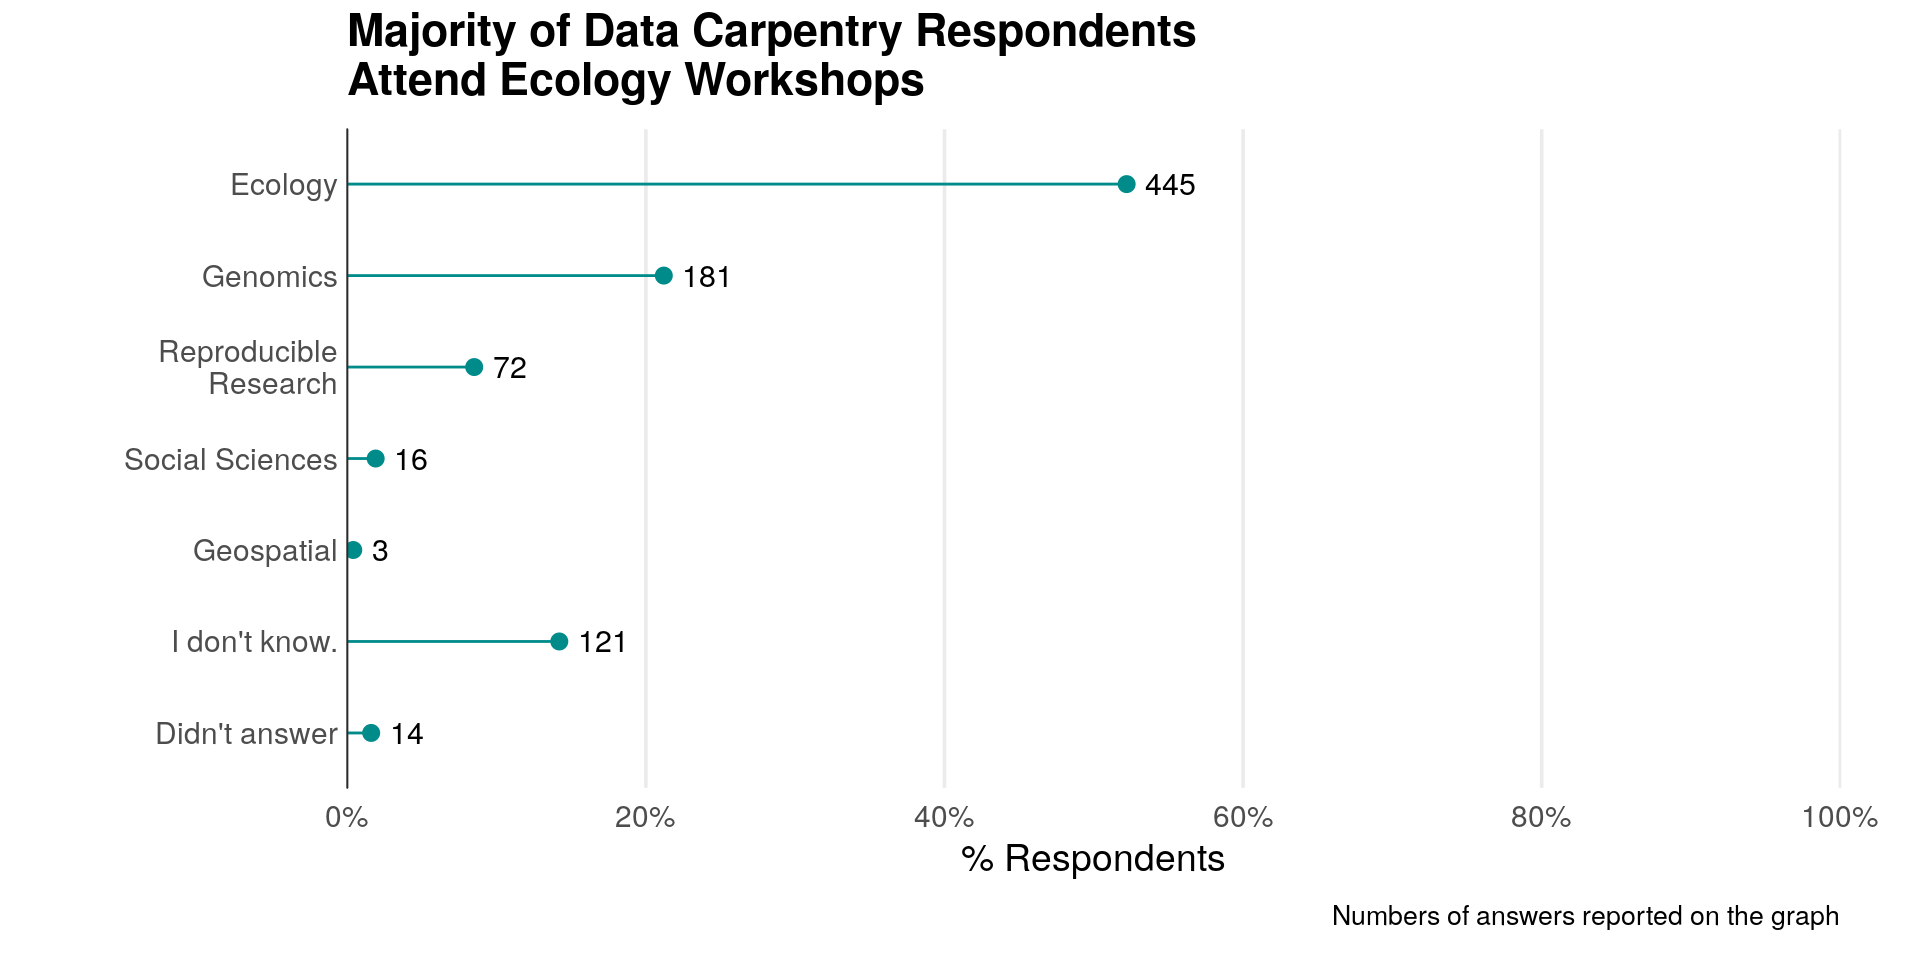
\includegraphics[width=\maxwidth]{../figures/dc-workshop-type-plot-1}

\begin{longtable}[]{@{}lrr@{}}
\toprule
Data Carpentry: Language Covered in Workshops & n & \%\tabularnewline
\midrule
\endhead
R & 614 & 71.9\tabularnewline
Python & 118 & 13.8\tabularnewline
Didn't answer & 60 & 7.0\tabularnewline
Neither & 57 & 6.7\tabularnewline
I don't know./I don't remember. & 5 & 0.6\tabularnewline
\bottomrule
\end{longtable}

As previously mentioned, Data Carpentry workshops are domain-specific,
and curricula include Ecology, Genomics, Geospatial, Social Sciences,
and Reproducible Research. 71.9\% of respondents learned R in workshops
at your institution, while 13.8\% learned Python.

\subsection{Perception of Workshop Environment and
Experience}\label{perception-of-workshop-environment-and-experience}

\subsubsection{Comfort of the
environment}\label{comfort-of-the-environment}

We hope you share in our committment to making participation in
workshops a harassment-free experience for everyone, regardless of who
learners are, where they are from, or what their experience is with the
tools we teach. We teach instructors to establish norms for interaction
by having, discussing, and enforcing a Code of Conduct so that your
workshops provide open and inclusive learning environments. 78.8\% of
Data Carpentry respondents from your workshops either agree or strongly
agree that they felt comfortable learning in their workshop environment,
and 91.7\% of Software Carpentry's respondents agreed or strongly agreed
that the workshop atmosphere was welcoming.

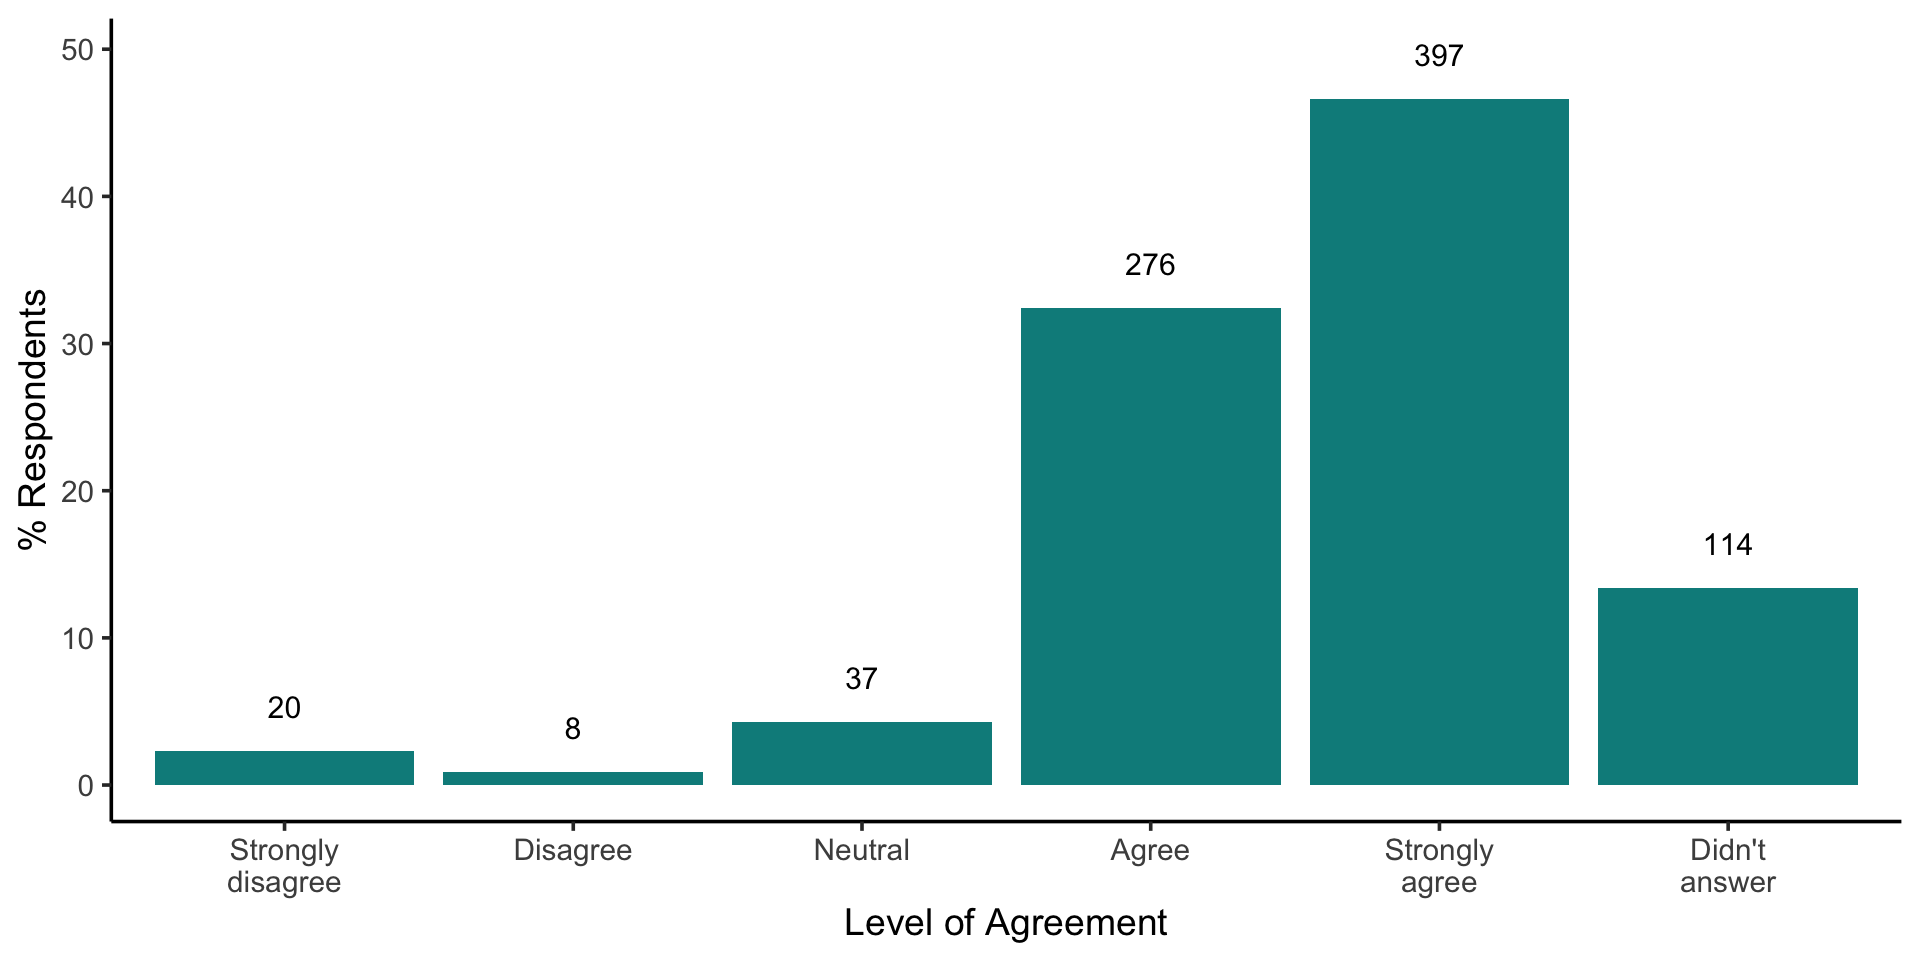
\includegraphics[width=\maxwidth]{../figures/dc-post-workshop-comfortable-environment-1}

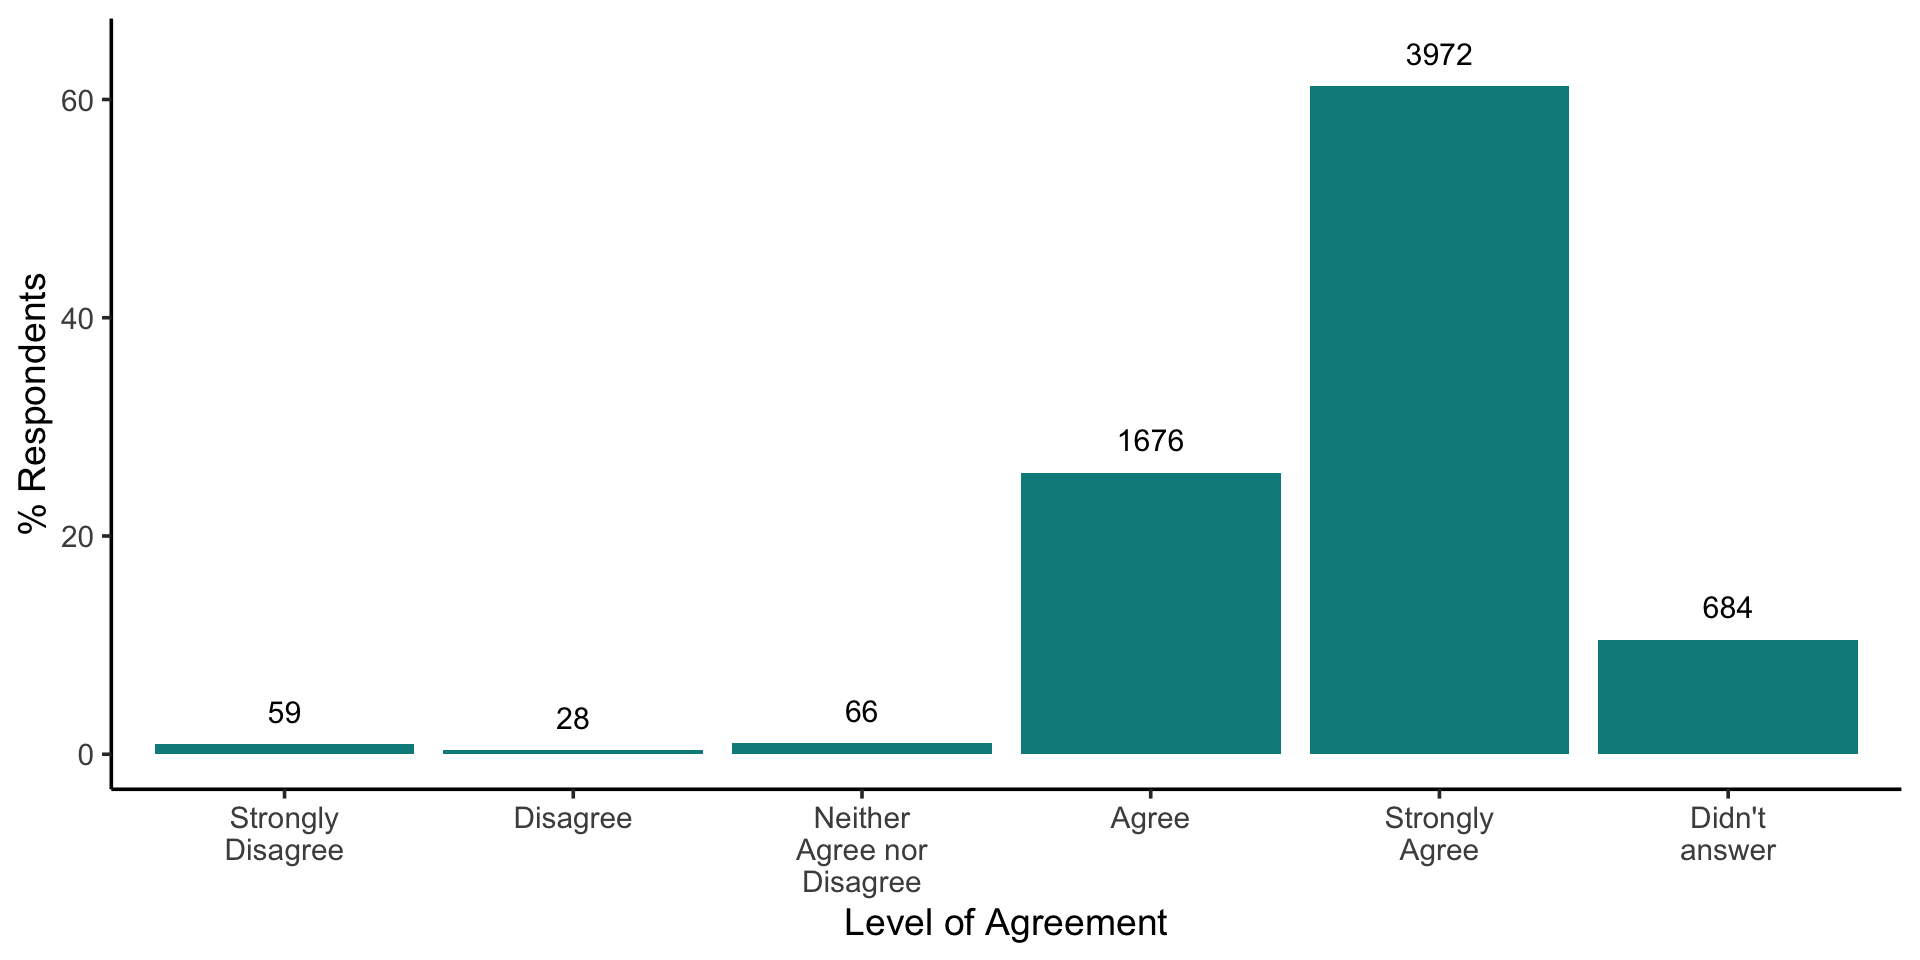
\includegraphics[width=\maxwidth]{../figures/swc-post-workshop-environment-1}

\subsubsection{Interaction with Instructors and
Helpers}\label{interaction-with-instructors-and-helpers}

Your Data Carpentry workshop respondents were asked to rate their level
of agreement with several statements regarding their instructors'
knowledge, instructional method, and enthusiasm. Their responses are in
the figure below, and axis labels correspond to the statements as
follows:

\begin{itemize}
\tightlist
\item
  \textbf{Instructors Knowledge}: The instructors were knowledgeable
  about the material being taught.
\item
  \textbf{Instructors Interacting}: I felt comfortable interacting with
  the instructors.
\item
  \textbf{Instructors Enthusiastic}: The instructors were enthusiastic
  about the workshop.
\item
  \textbf{Instructors Clear Answers}: I was able to get clear answers to
  my questions from the instructors.
\end{itemize}

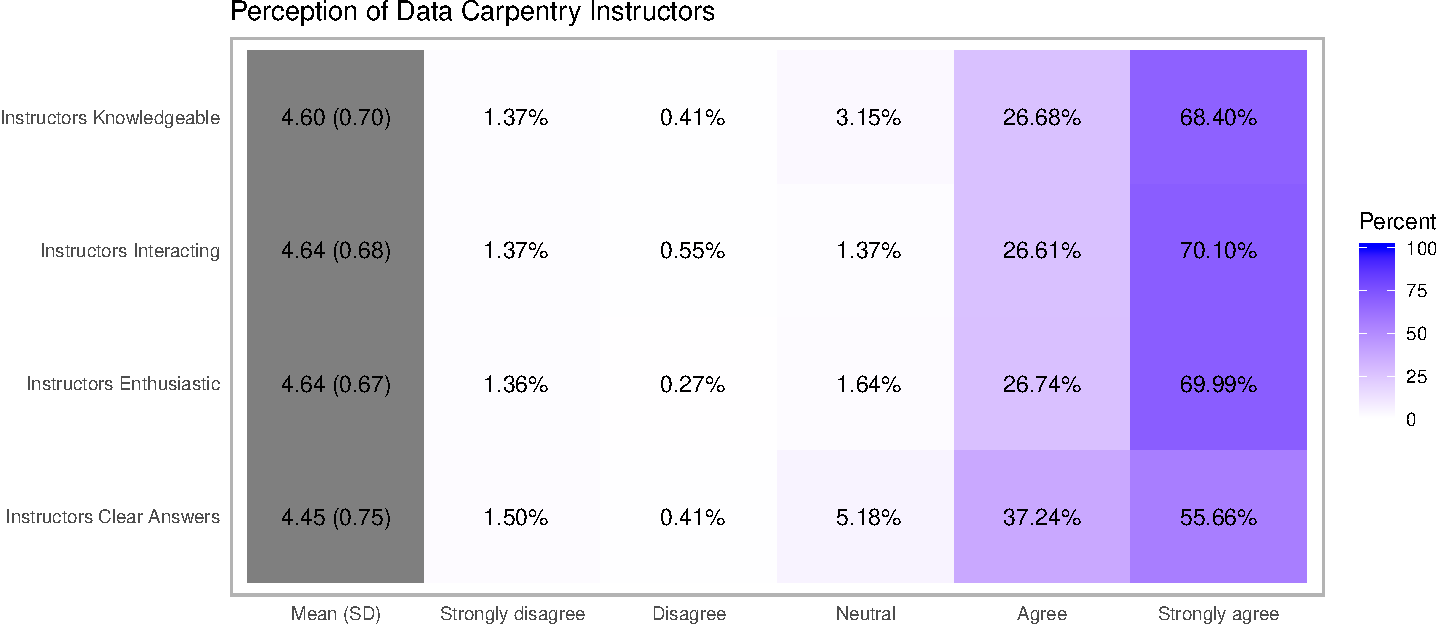
\includegraphics[width=\maxwidth]{../figures/dc-perception-instructors-heatmap-1}

96.2\% of respondents said they felt comfortable interacting with the
instructors. 94.8\% and 96.7\% of respondents felt your instructors were
knowledgeable about the material being taught, and were enthusiastic
about the workshop, respectively. Lastly, 92.9\% of respondents felt
they were able to get clear answers to their questions from their
instructors.

Software Carpentry respondents were asked to rate how they felt
instructors and helpers worked as a team, based on the following
criteria:

\begin{itemize}
\tightlist
\item
  \textbf{Considerate}: Instructors/Helpers were considerate.
\item
  \textbf{Enthusiastic}: Instructors/Helpers were enthusiastic.
\item
  \textbf{Clear Answers}: Instructors/Helpers gave clear answers to your
  questions.
\item
  \textbf{Communicators}: Instructors/Helpers were good communicators.
\end{itemize}

The two neutral centered plots below provide an analysis of respondent's
answers for both instructors and helpers.

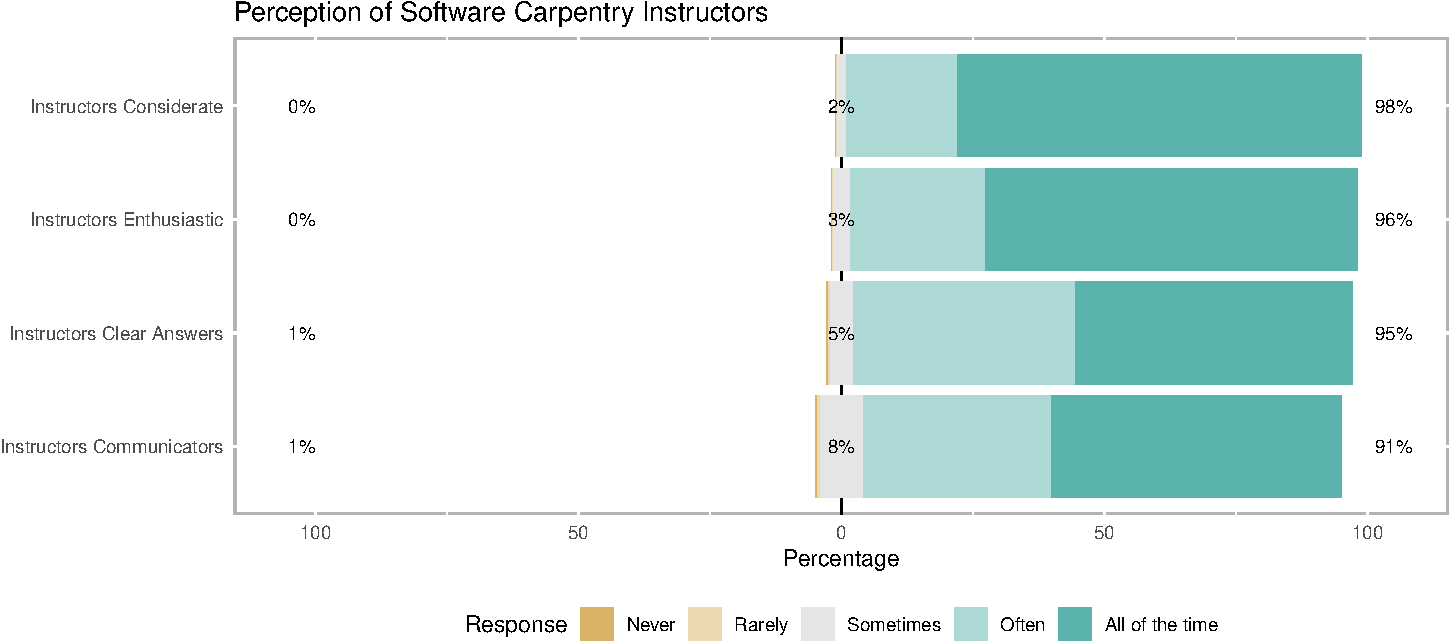
\includegraphics[width=\maxwidth]{../figures/swc-perception-instructors-1}

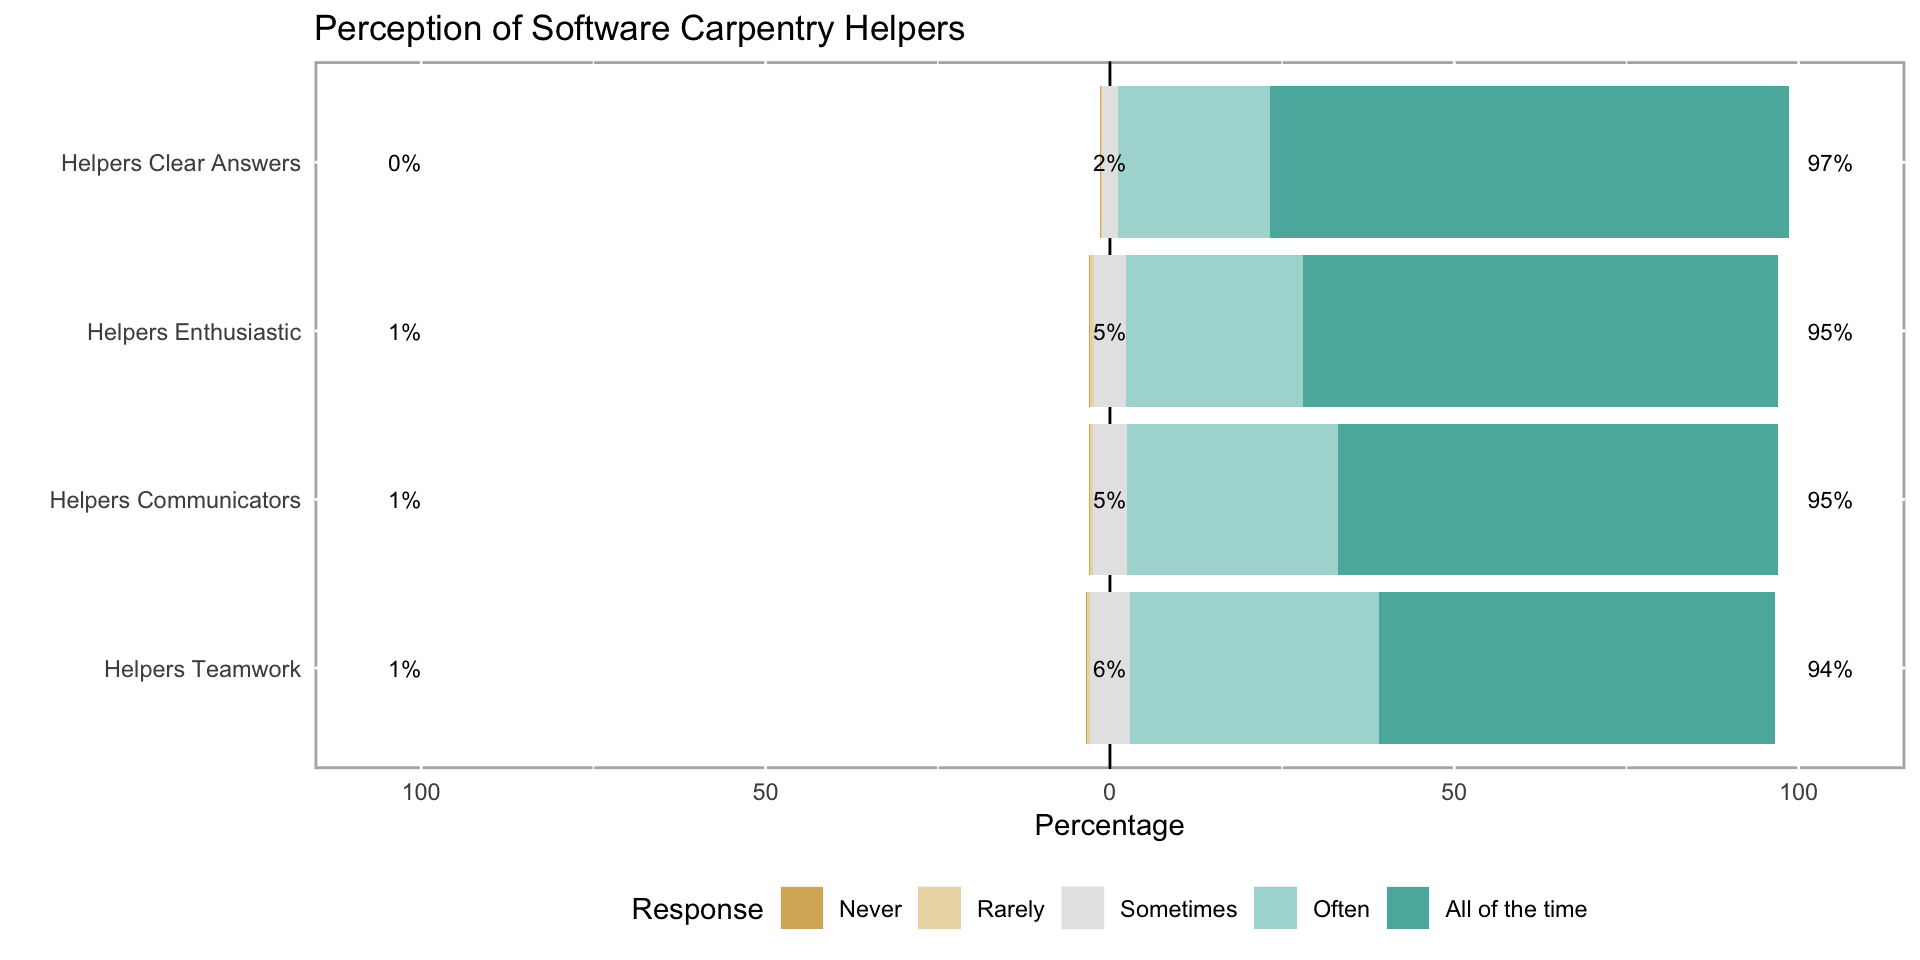
\includegraphics[width=\maxwidth]{../figures/swc-perception-helpers-1}

\subsection{Applicability of the skills
learned}\label{applicability-of-the-skills-learned}

One of the goals for Data Carpentry's lessons is that learners are able
to immediately apply what they learned at the workshop. The figure below
shows that 65\% either agree or strongly agree that they were able to
apply what they learned immediately after attending a workshop at your
institution.

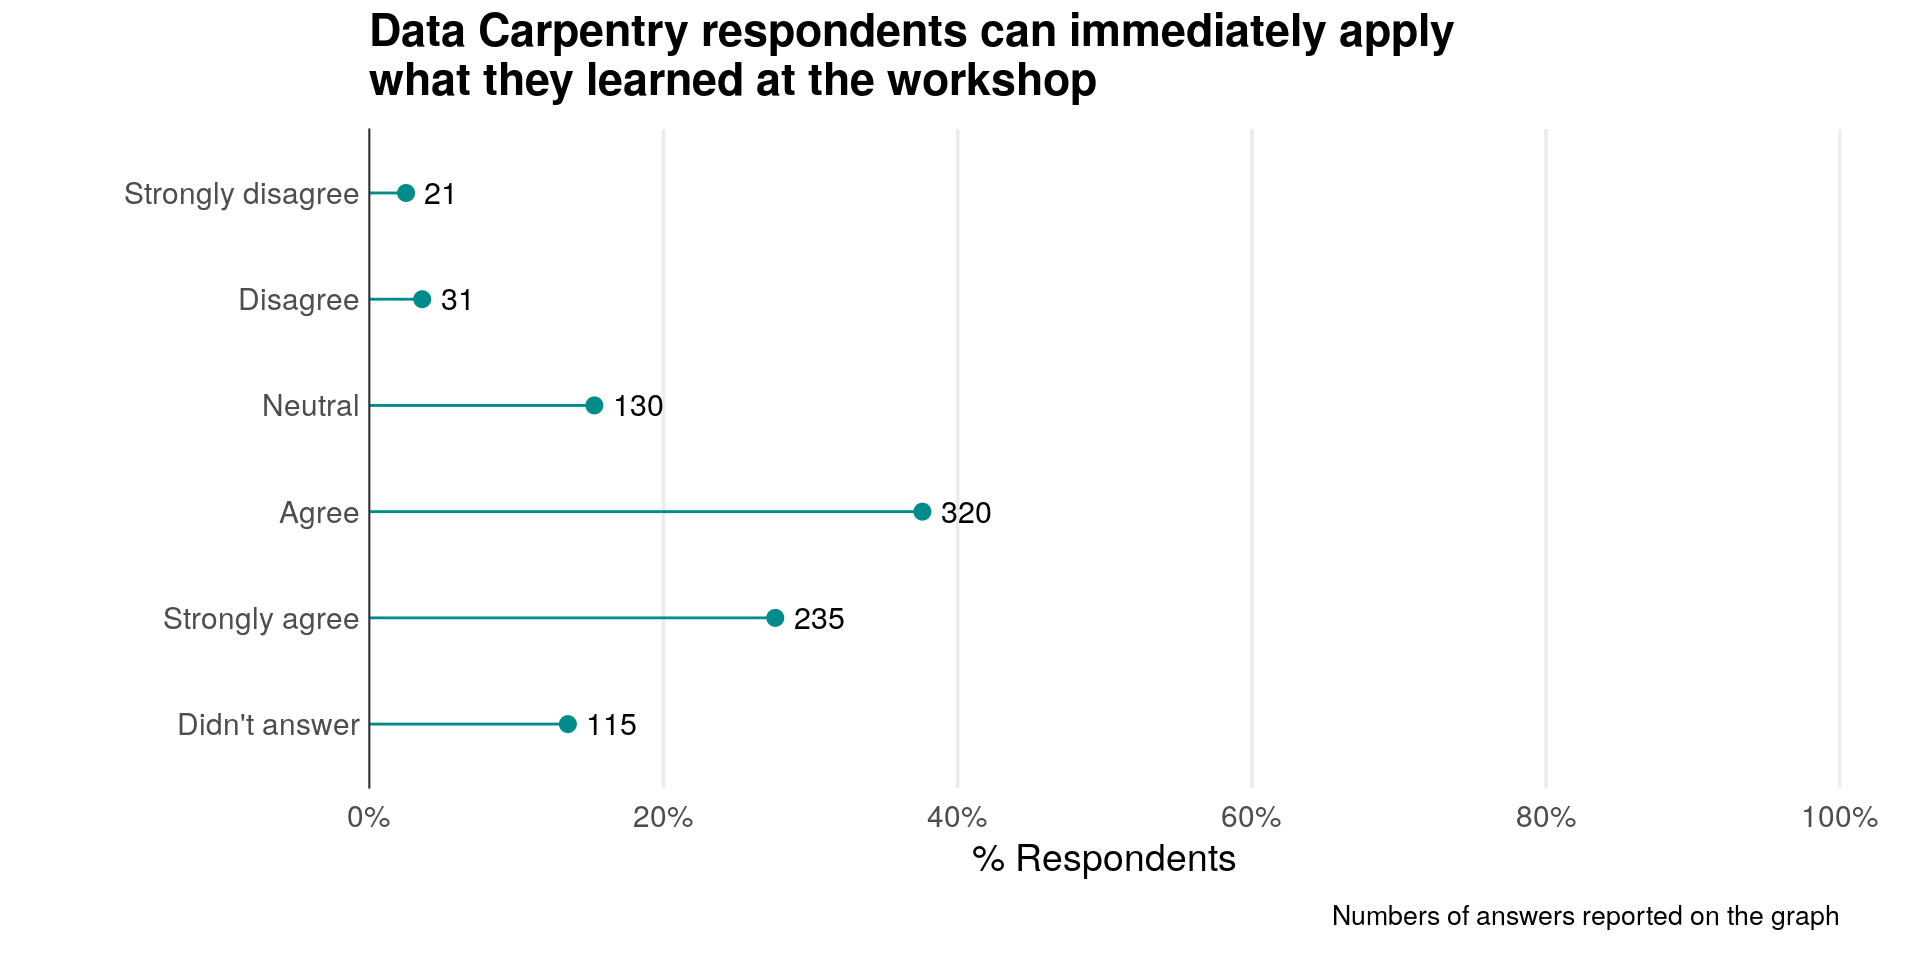
\includegraphics[width=\maxwidth]{../figures/dc-skill-applicability-plot-1}

\subsection{Was the information covered in the workshops
new?}\label{was-the-information-covered-in-the-workshops-new}

49.6\% of your Software Carpentry workshop learners either learned
mostly or all new information during the workshop they attended, while
another 20.3\% learned something new.

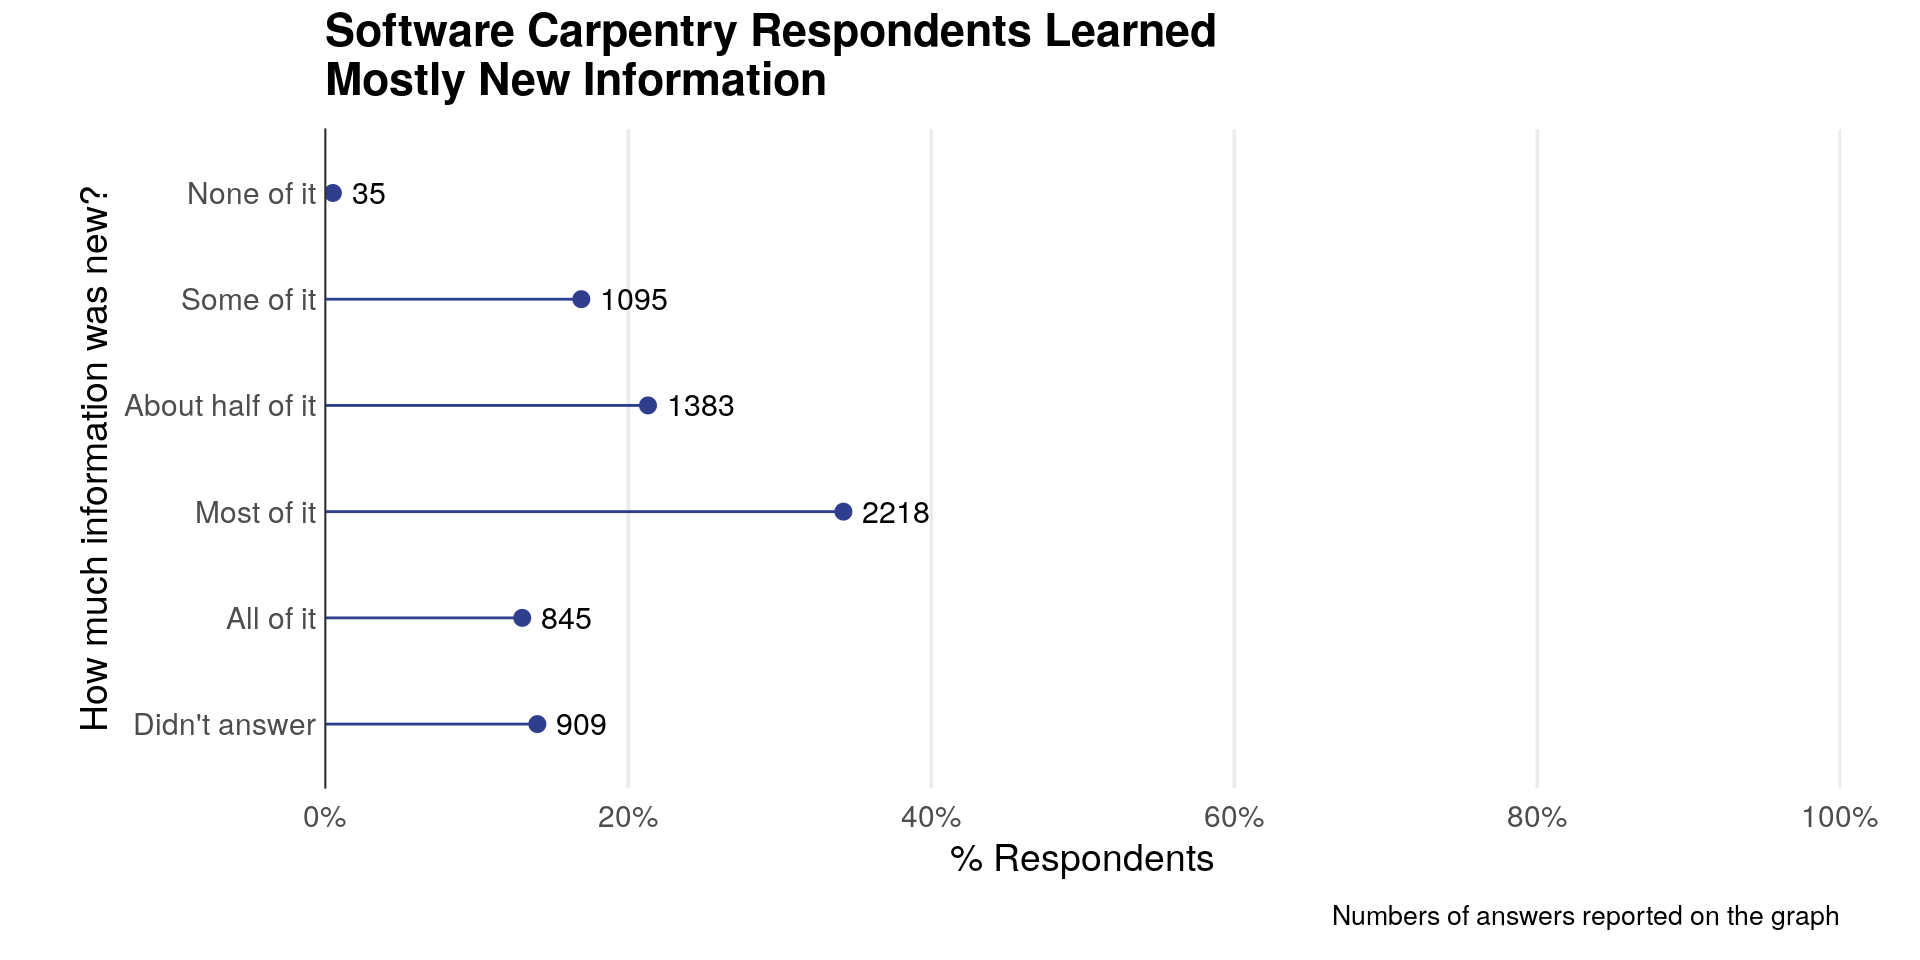
\includegraphics[width=\maxwidth]{../figures/swc-new-information-plot-1}

\subsection{Workshop Experience}\label{workshop-experience}

\begin{longtable}[]{@{}lrr@{}}
\toprule
Data Carpentry Respondents Having Accessibility Issues & n &
\%\tabularnewline
\midrule
\endhead
Yes & 79 & 9.3\tabularnewline
No & 654 & 76.6\tabularnewline
Didn't answer & 121 & 14.2\tabularnewline
\bottomrule
\end{longtable}

Both Data Carpentry and Software Carpentry learners were asked to inform
workshop organizers if there was anything they needed to make their
workshop experience better. Data Carpentry's respondents were asked if
they had accessibility issues, and 9.3\% reported they did. We recommend
that you read through the open-ended responses included in the raw data
to address any concerns regarding accessibility issues.

\subsection{Net Promoter Score}\label{net-promoter-score}

We use the \href{https://en.wikipedia.org/wiki/Net_Promoter}{Net
Promoter Score} to measure learners' likelihood of recommending
workshops to a friend or colleague. The scoring for this question is on
a 0 to 100 scale. Respondents scoring from 0 to 64 are labeled
\emph{Detractors}, and are believed to be less likely to recommend a
workshop. Those who respond with a score of 85 to 100 are called
\emph{Promoters}, and are considered likely to recommend a workshop.
Respondents between 65 and 84 are labeled \emph{Passives}, and their
behavior falls between Promoters and Detractors.

\begin{longtable}[]{@{}lrr@{}}
\toprule
Data Carpentry Net Promoter Score & n & \%\tabularnewline
\midrule
\endhead
Detractor & 32 & 3.7\tabularnewline
Passive & 131 & 15.3\tabularnewline
Promoter & 565 & 66.2\tabularnewline
Didn't answer & 126 & 14.8\tabularnewline
\bottomrule
\end{longtable}

77.6\% of your Data Carpentry respondents who answered this question are
promoters (i.e.~would recommend a workshop).

For Software Carpentry respondents who answered this questions, 57.8\%
are promoters.

\subsection{Effect of Workshops on Learners Self-Reported Perspectives:
Skills \&
Confidence}\label{effect-of-workshops-on-learners-self-reported-perspectives-skills-confidence}

Your learners were asked to rate their level of agreement with the
following statements related to Data Carpentry's workshop goals and
learning objectives. The figure below provides a visual representation
of their responses, comparing them before the workshop and after the
workshop. Axis labels and the corresponding question are organized
around 3 themes as follows:

\begin{itemize}
\tightlist
\item
  Efficiency:

  \begin{itemize}
  \tightlist
  \item
    \textbf{Write Program}: I can write a small program/script/macro to
    solve a problem in my own work.
  \item
    \textbf{Programming Efficient}: Using a programming language (like R
    or Python) can make me more efficient at working with data.
  \end{itemize}
\item
  Reproducibility:

  \begin{itemize}
  \tightlist
  \item
    \textbf{Raw Data}: Having access to the original, raw data is
    important to be able to repeat an analysis.
  \item
    \textbf{Analyses Easier}: Using a programming language (like R or
    Python) can make my analyses easier to reproduce.
  \end{itemize}
\item
  Self-efficacy

  \begin{itemize}
  \tightlist
  \item
    \textbf{Search Online}: I know how to search for answers to my
    technical questions online.
  \item
    \textbf{Overcome Problem}: While working on a programming project,
    if I get stuck, I can find ways of overcoming the problem.
  \item
    \textbf{Programming Confident}: I am confident in my ability to make
    use of programming software to work with data.
  \end{itemize}
\end{itemize}

The scoring for the above factors ranges from strongly disagree (1) to
strongly agree (5).

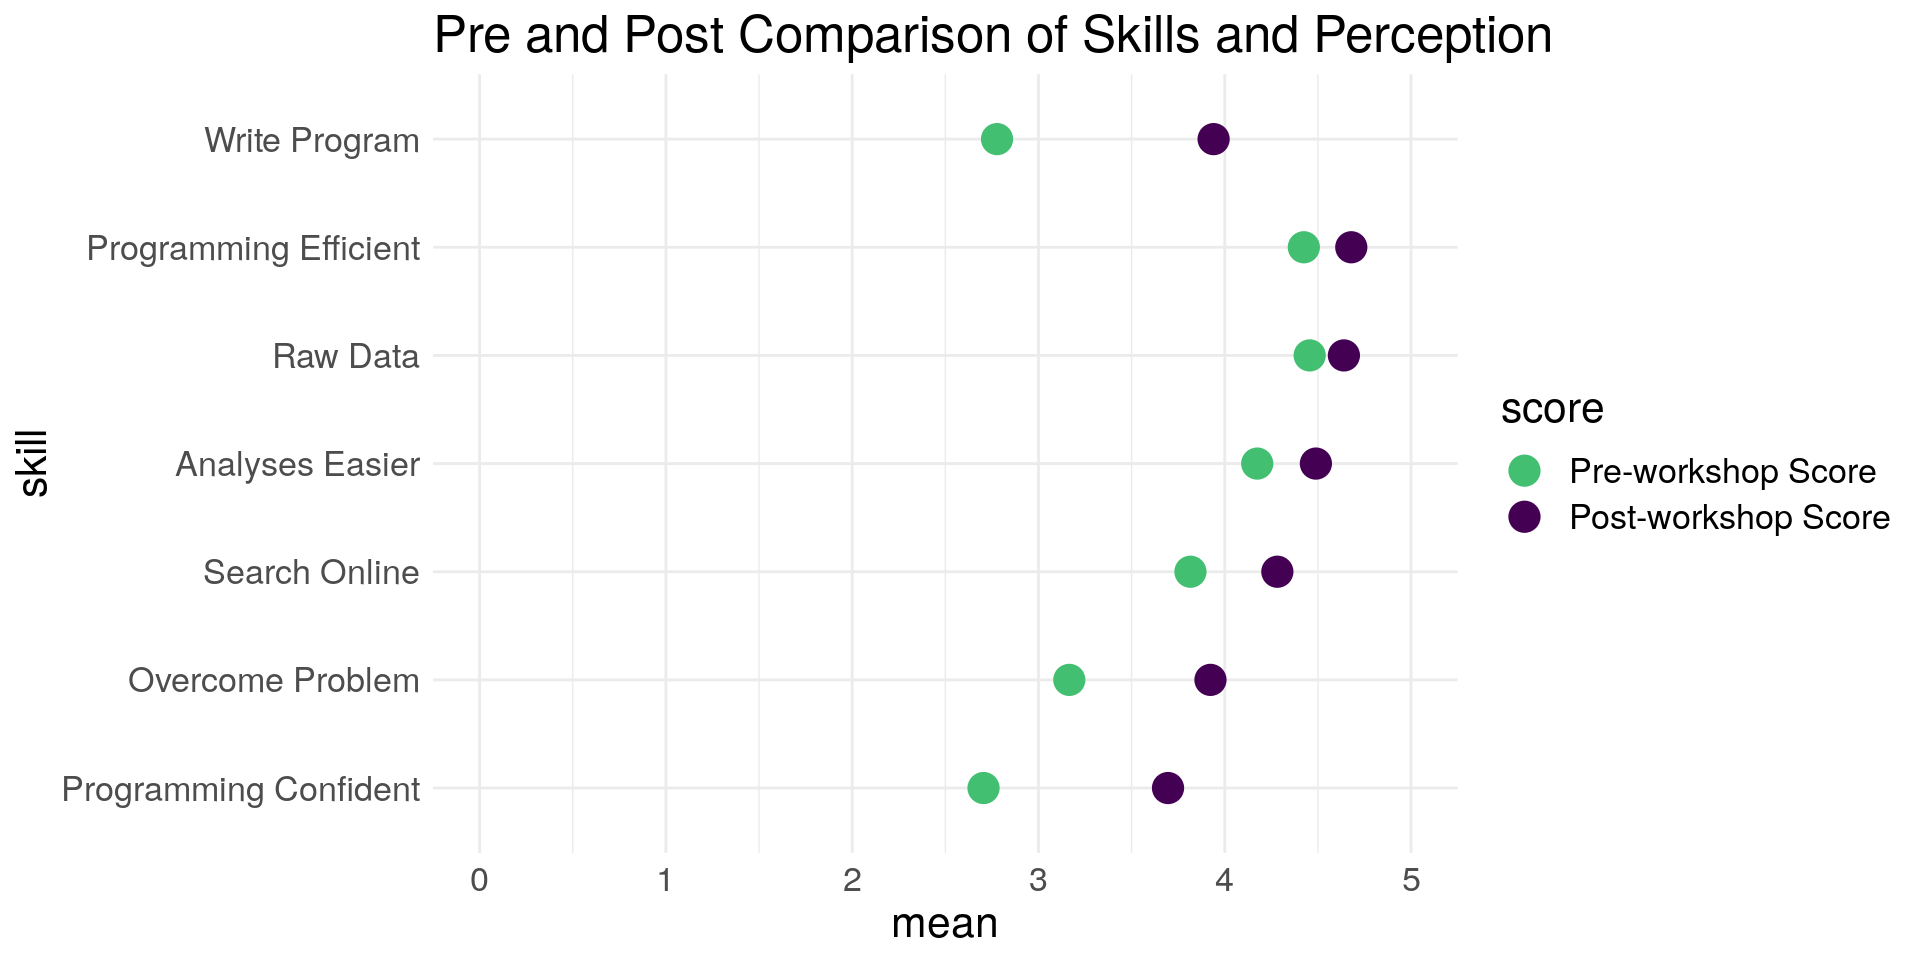
\includegraphics[width=\maxwidth]{../figures/dc-paired-data-mean-1}

The comparison above is paired, meaning, we are comparing those who
provided us with a unique identifier and who completed both the pre- and
post-workshop survey. This figure includes 411 responses.

In the figures below, we show another representation of the pre- and
post-comparison of respondents skills and perspectives. The figures
below include the data for all learners, not only those who provided a
unique identifier \emph{and} took both the pre- and post-workshop
surveys.

The neutral centered graphs below provide an even clearer picture of the
shift in respondents' self-reported confidence and skills.

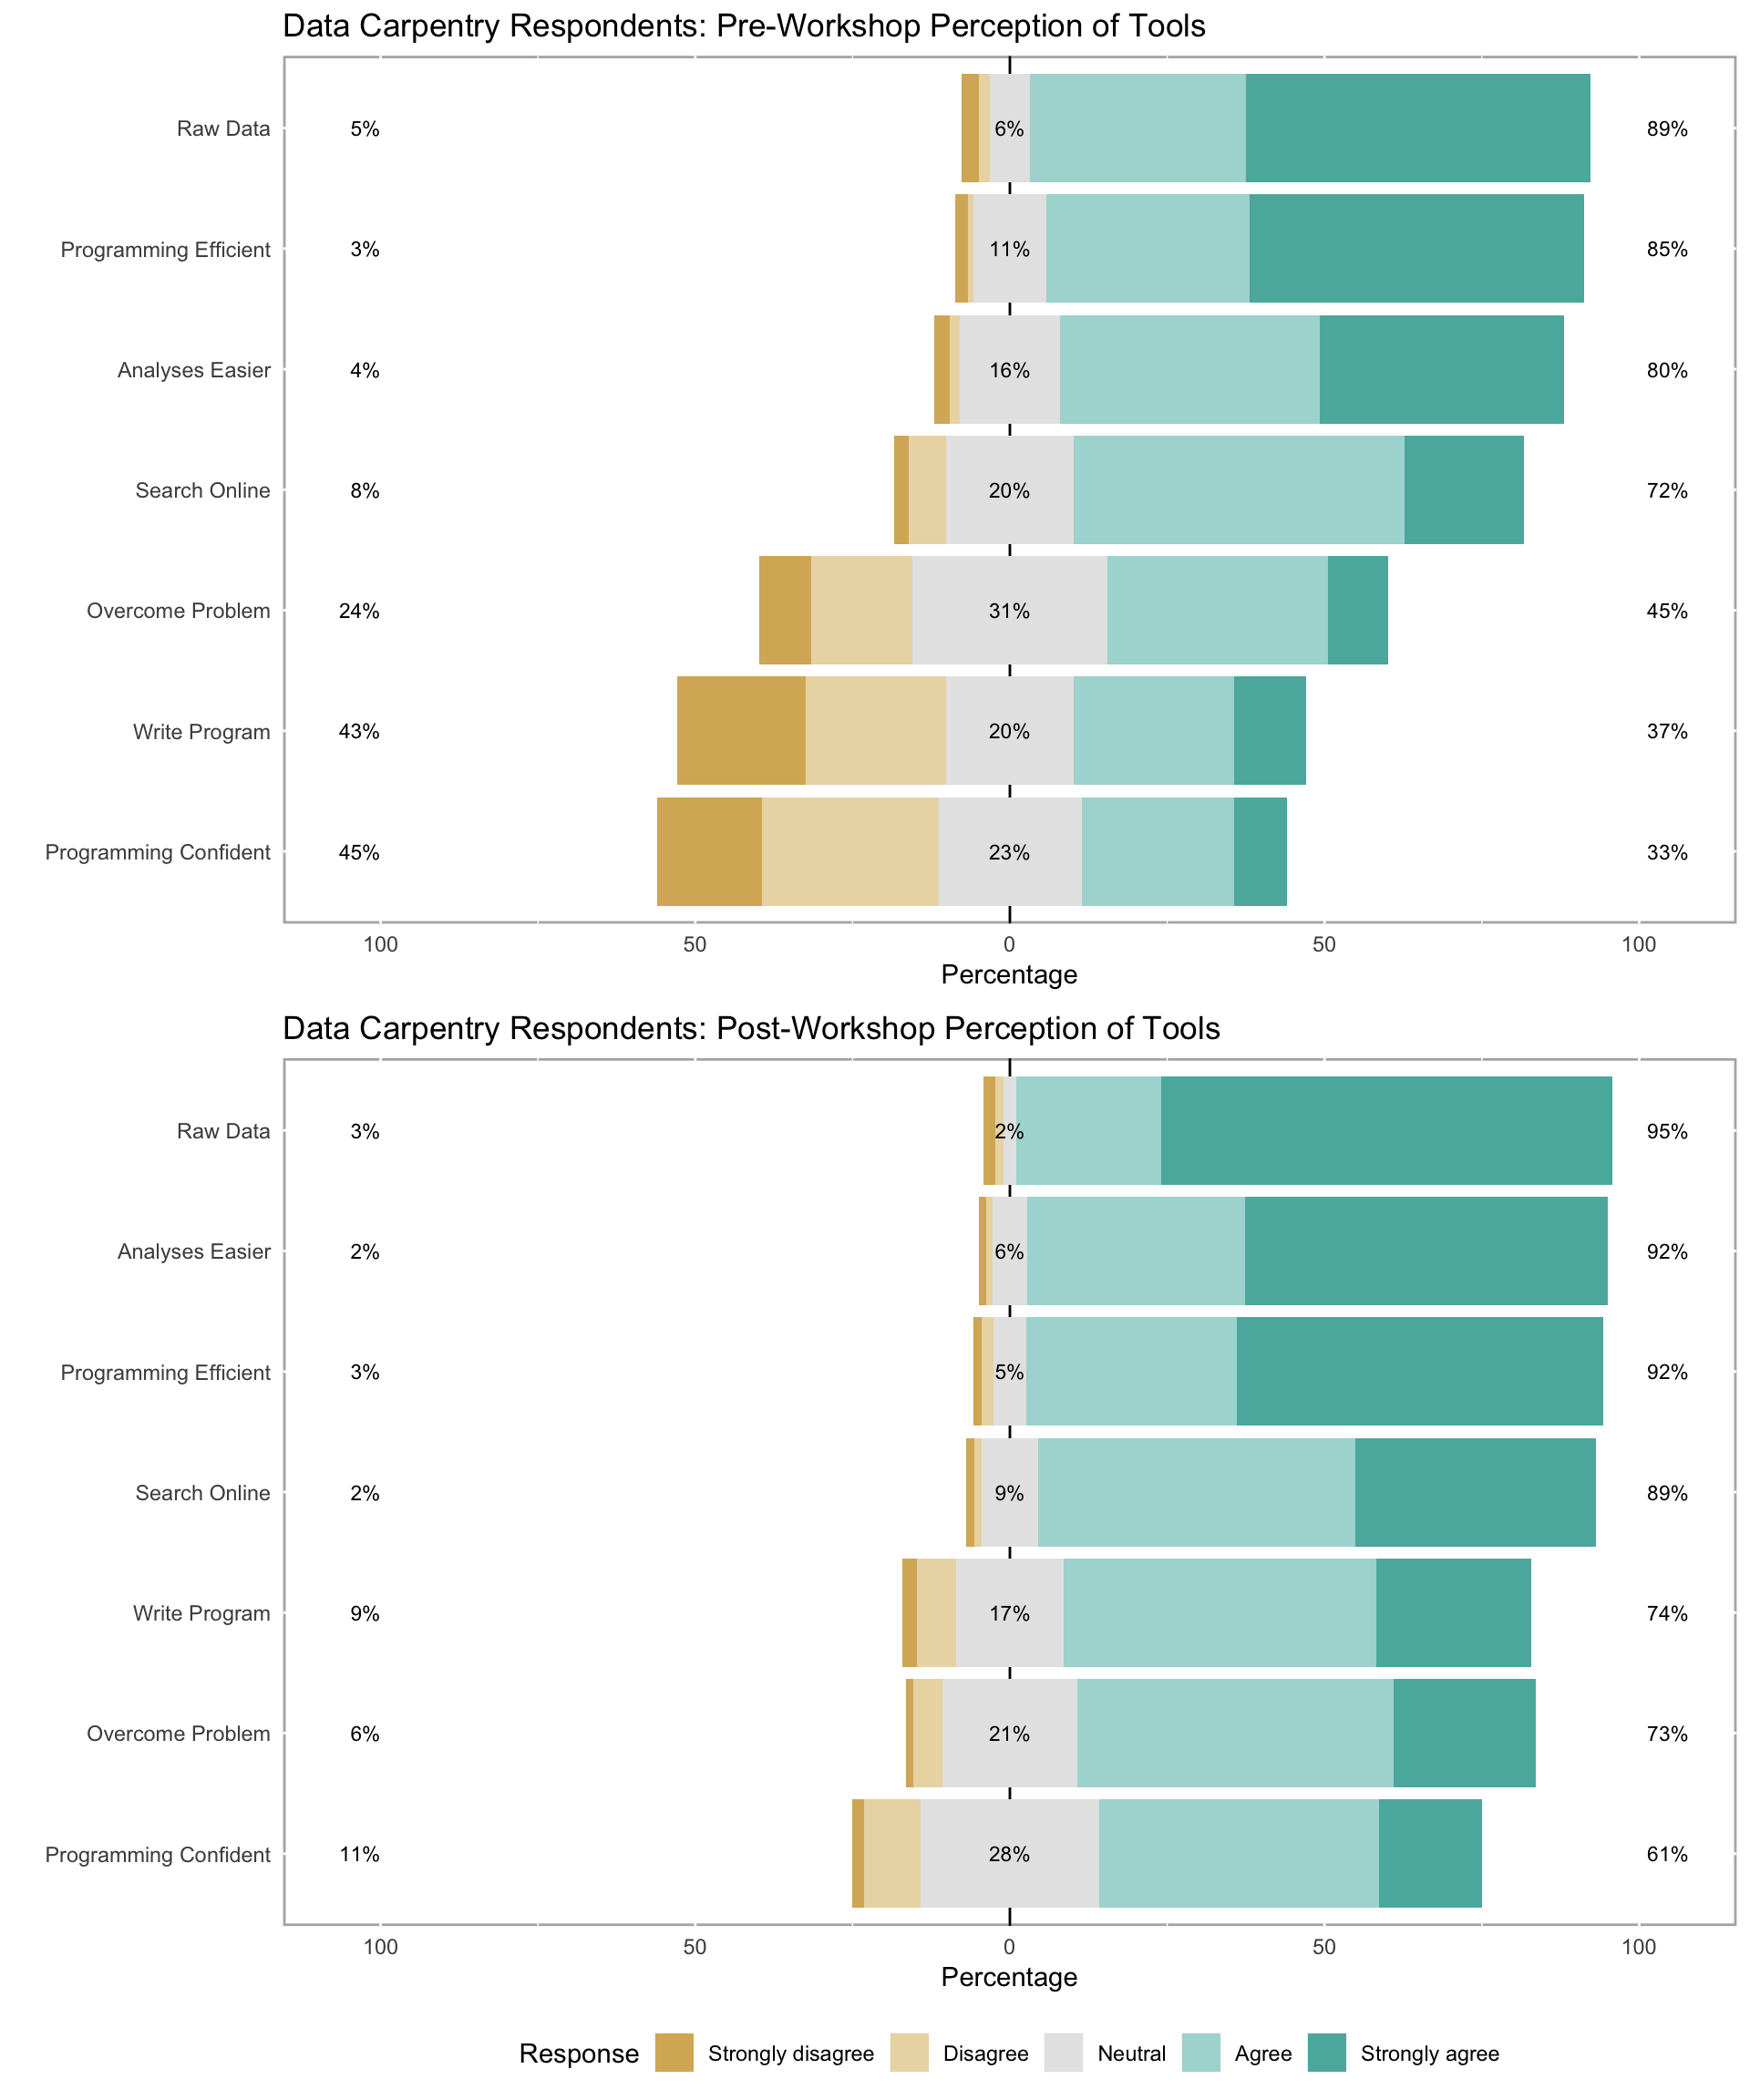
\includegraphics[width=\maxwidth]{../figures/dc-tools-perception-1}

Software Carpentry Respondents were asked to tell us about their
experience with these topics before the workshop:

\begin{itemize}
\tightlist
\item
  R
\item
  Unix Shell
\item
  SQL
\item
  Python
\item
  Version Control with Git
\end{itemize}

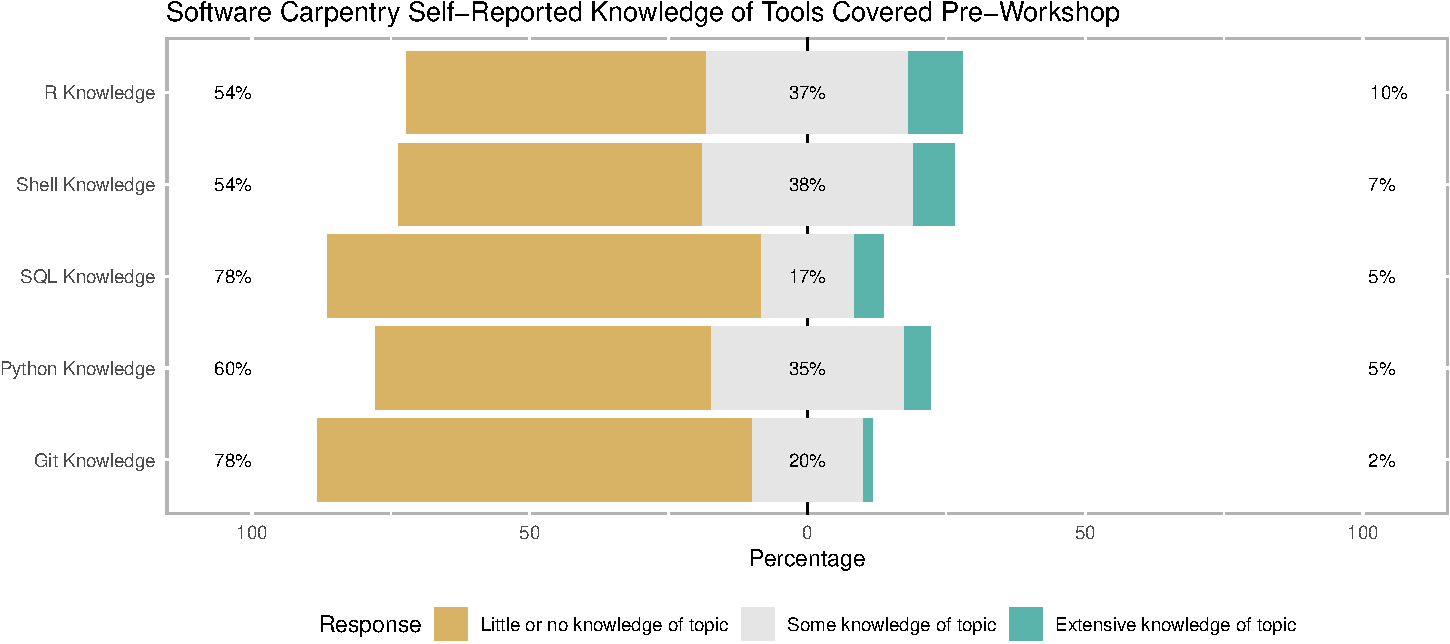
\includegraphics[width=\maxwidth]{../figures/swc-pre-tools-1}

From the figure, we see that your learners consider themselves beginners
from the topics covered in your workshops. When asked their knowledge of
the tools covered in their workshops, they rated their knowledge as
extensive from 1\% to 11\% for ``Git Knowledge'' and ``R Knowledge''.

The following is a comparison of your Software Carpentry respondents'
knowledge about the tools before compared to after the workshop.

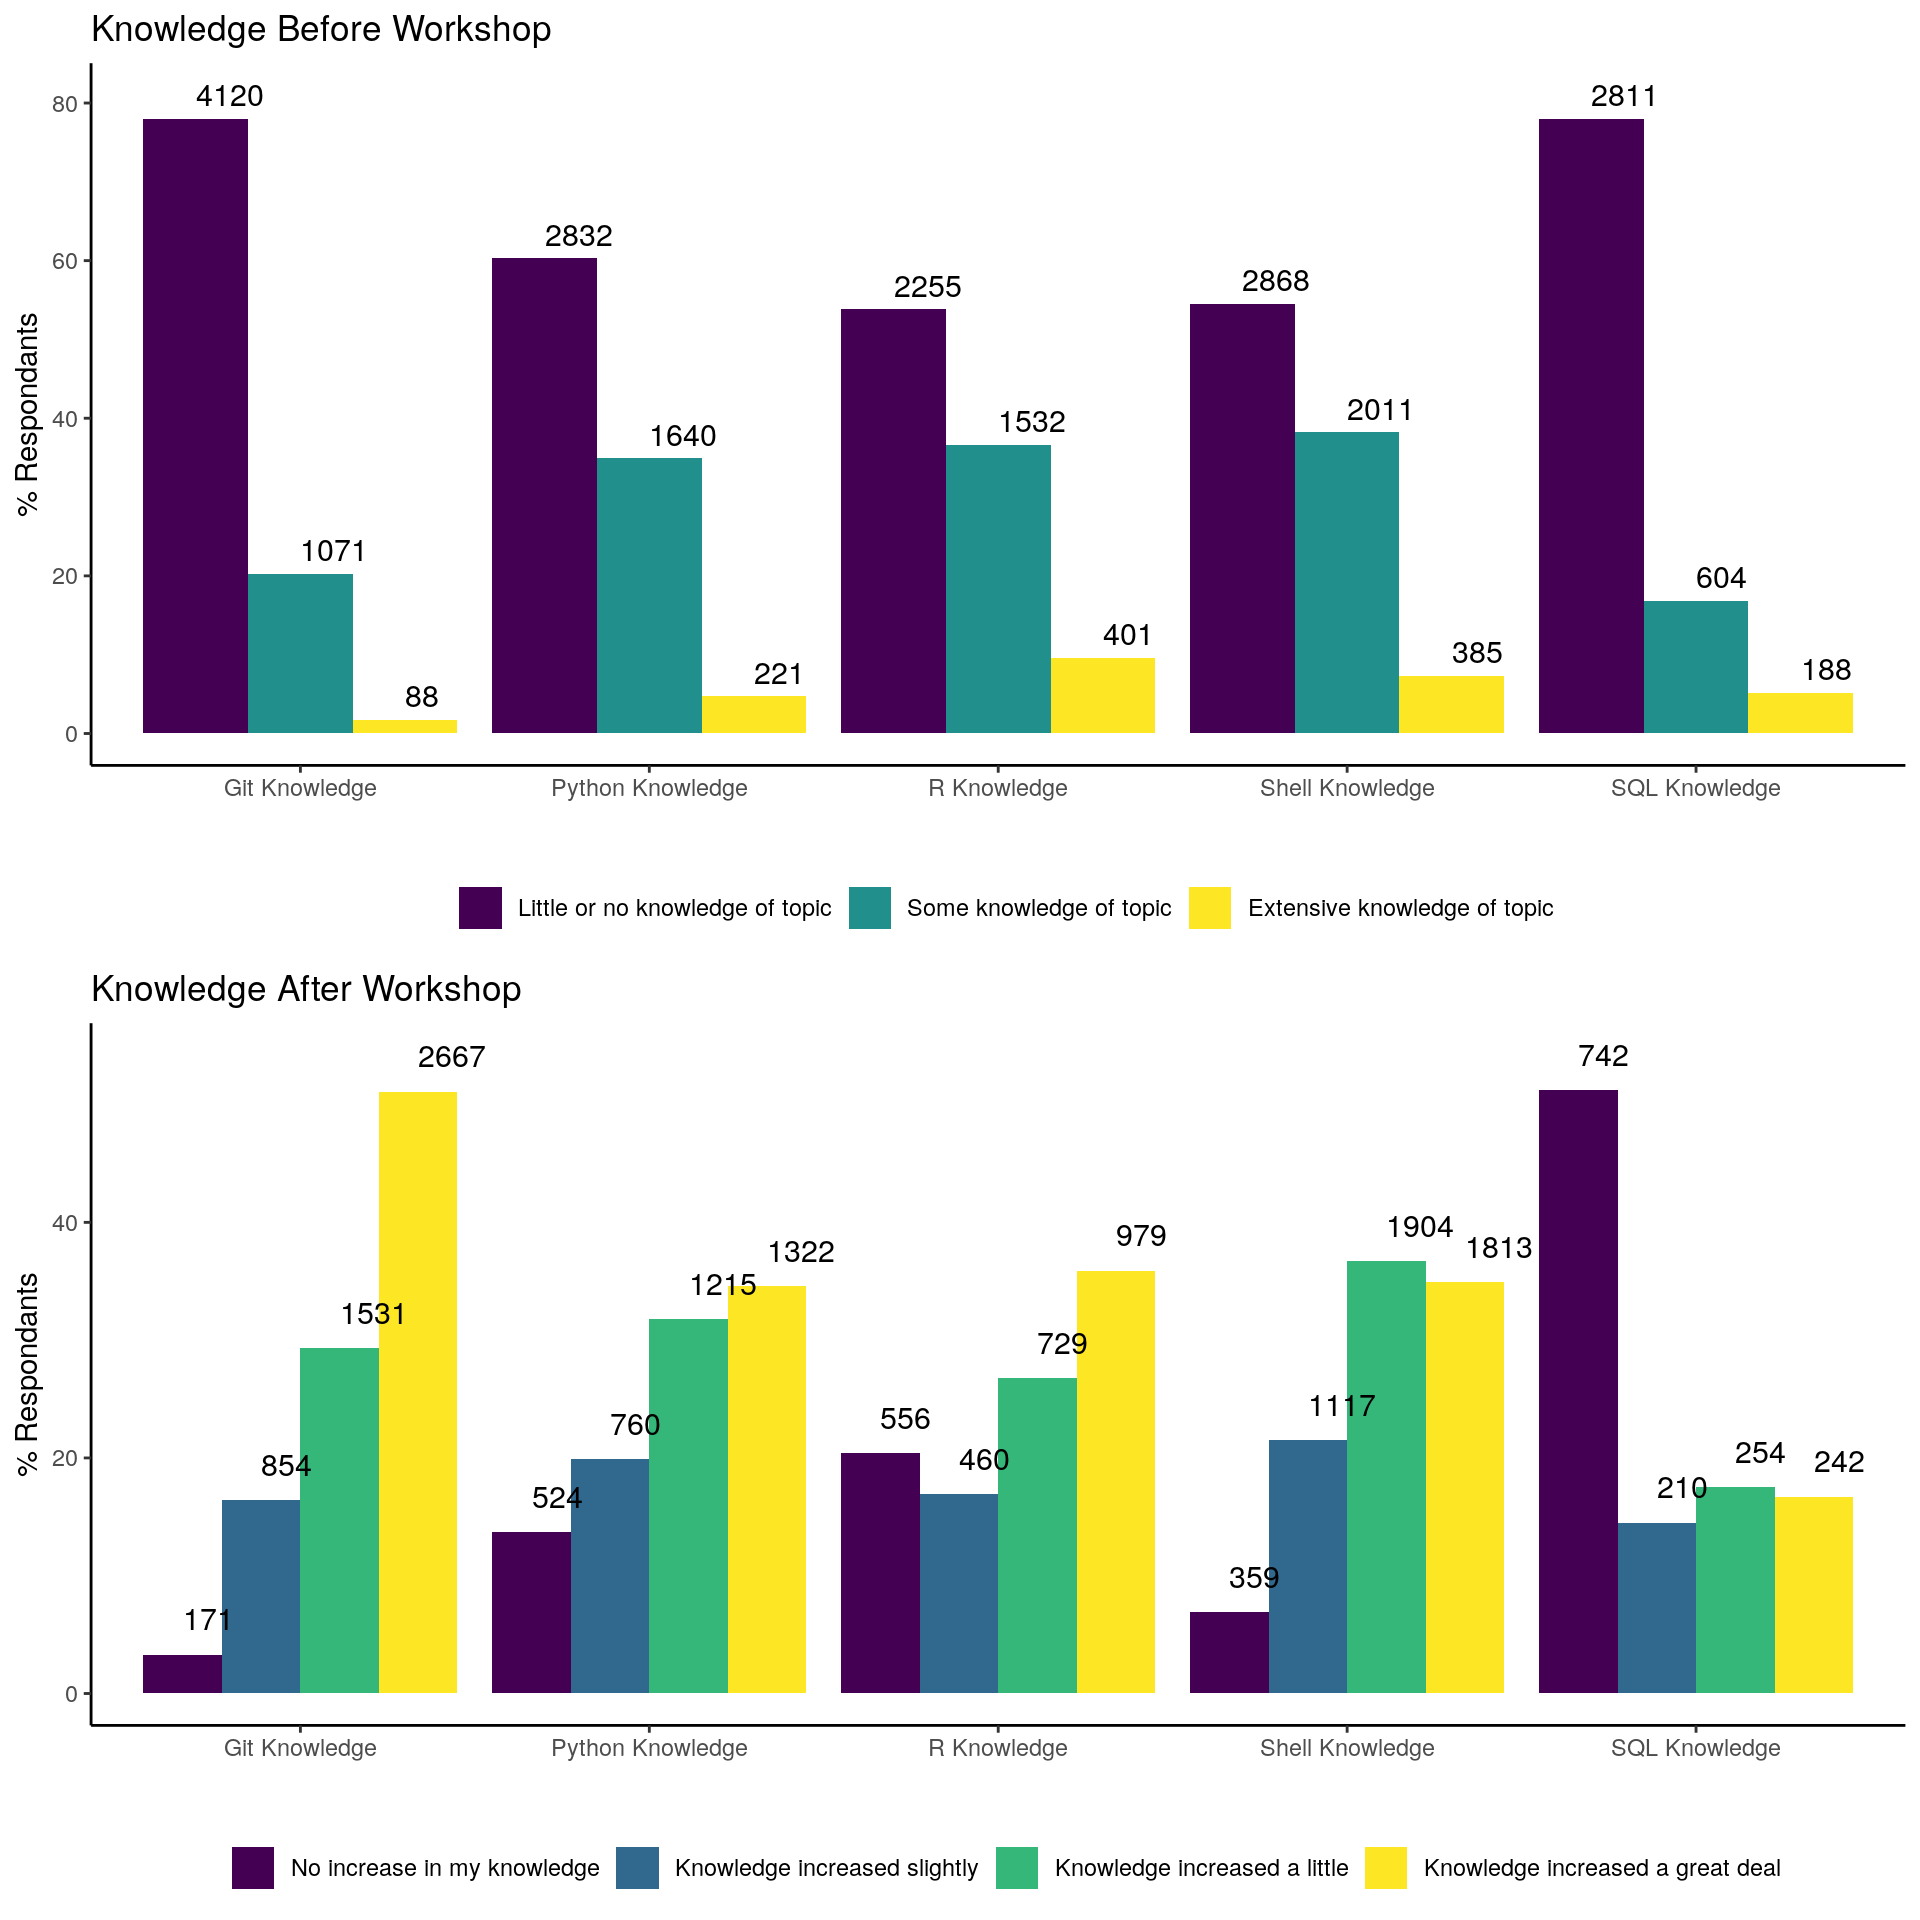
\includegraphics[width=\maxwidth]{../figures/swc-knowledge-change-1}

\subsubsection{Respondent Ability to Perform Computing
Tasks}\label{respondent-ability-to-perform-computing-tasks}

Motivation is important, but being confident in your ability to complete
specific computing tasks is an equally important goal of Software
Carpentry. The grid below shows respondents' self-reported ability to
complete tasks including:

\begin{itemize}
\tightlist
\item
  \textbf{Pipes}: Using pipes to connect shell commands
\item
  \textbf{Loops}: Writing a `for loop' to automate tasks\\
\item
  \textbf{Git}: Initializing a repository with git
\item
  \textbf{Function}: Writing a function
\item
  \textbf{Import Library}: Importing a library or package in R or Python
\item
  \textbf{Unit Test}: Writing a unit test in Python or R
\item
  \textbf{SQL Query}: Writing an SQL query
\end{itemize}

It also provides their self-reported level of confidence in being able
to complete the tasks above after completing the workshop.

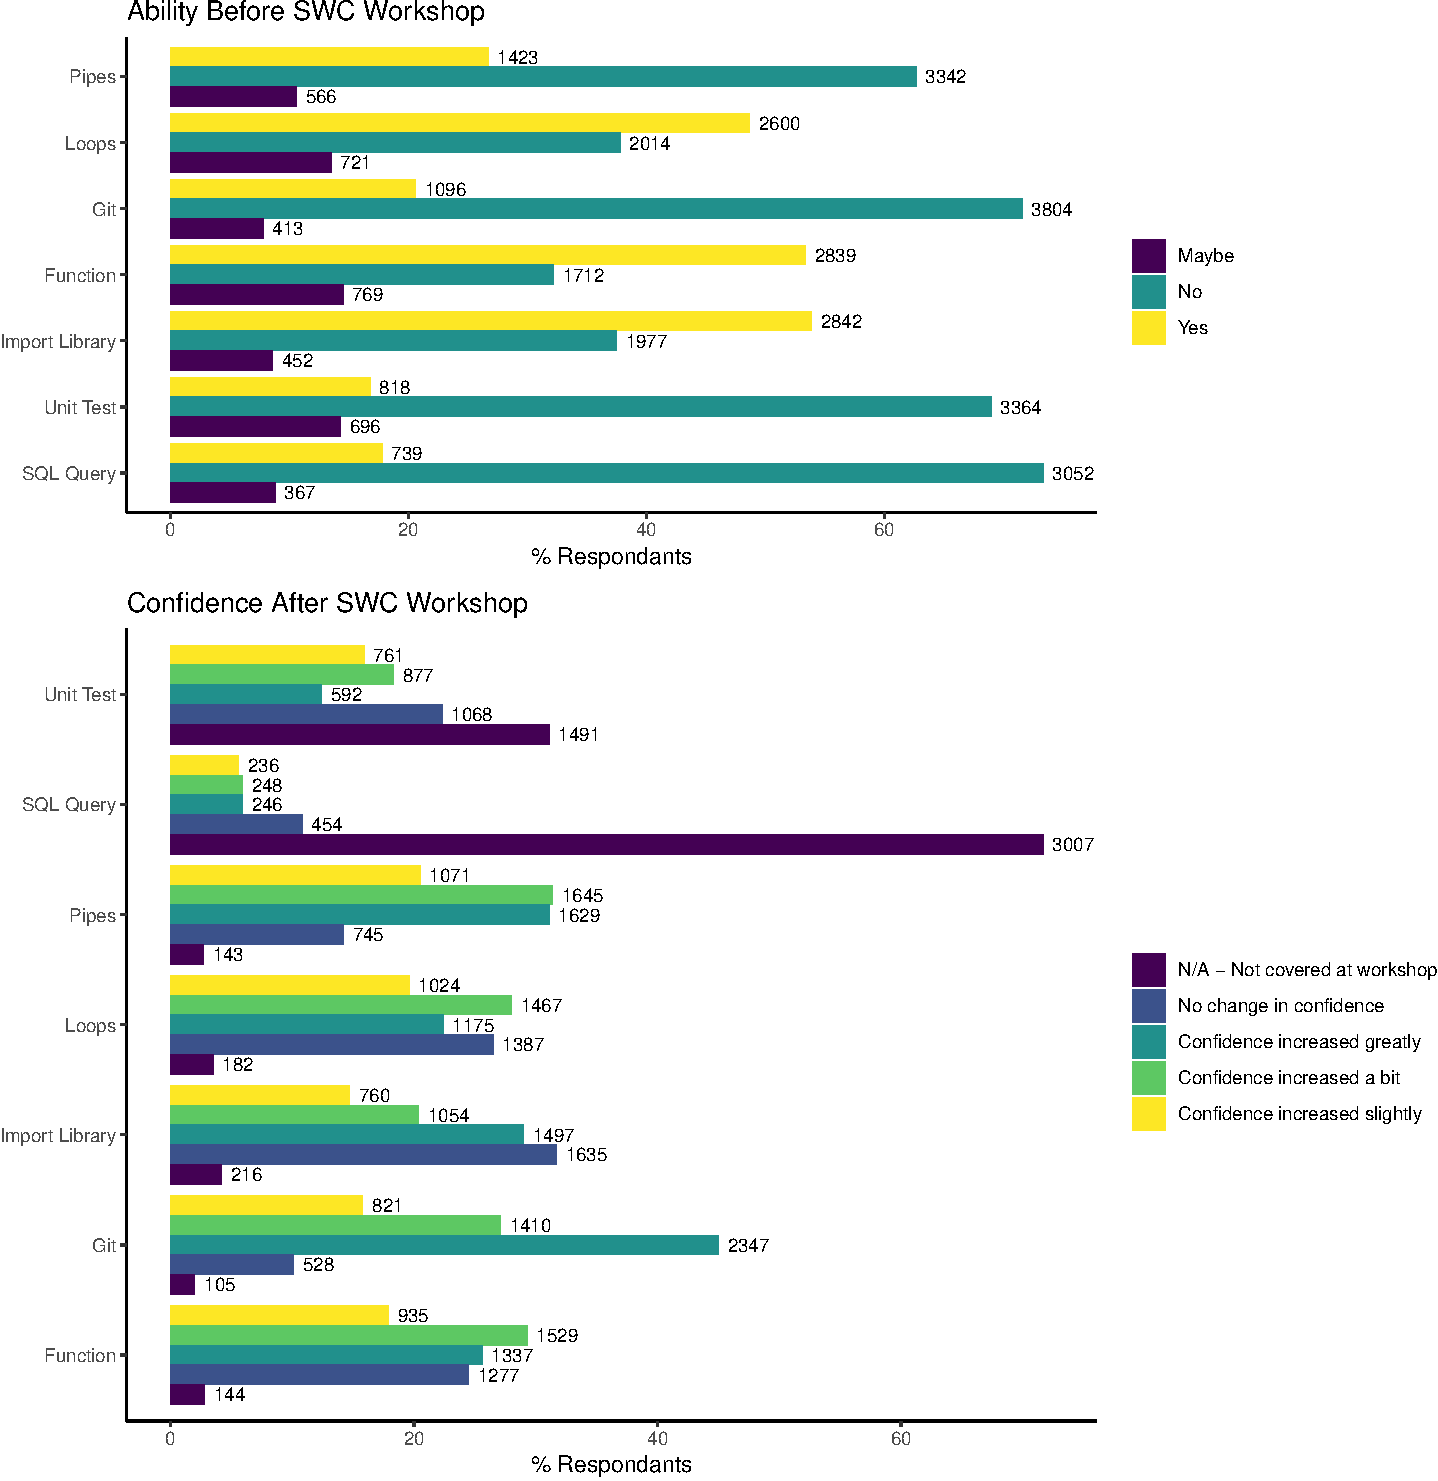
\includegraphics[width=\maxwidth]{../figures/swc-ability-confidence-1}

These figures tell us that, before the workshop, between 27.1\% and
69.6\% of the respondents did not feel they could initialize a
repository in Git, write a `for loop' to automate tasks, use pipes to
connect shell commands, write a SQL query, and/or write a unit test in R
or Python. 26.3\% of learners felt their confidence increased greatly
with respect to importing a library or package in R or Python.

In summary, we hope that you will use the figures above as a resource to
make the case to continue organizing Software and Data Carpentry
workshops at your institution.

\subsection{Demographics}\label{demographics}

\subsubsection{Learners' discipline}\label{learners-discipline}

The distribution of your learners by discipline is provided below for
both Data and Software Carpentry workshops held at your institution.

\begin{longtable}[]{@{}lrr@{}}
\toprule
Data Carpentry's Respondents by Discipline & n & \%\tabularnewline
\midrule
\endhead
Life Sciences & 444 & 35.6\tabularnewline
Agricultural or Environmental Sciences & 307 & 24.6\tabularnewline
Bioinformatics/Genomics & 292 & 23.4\tabularnewline
Biomedical/Health Sciences & 288 & 23.1\tabularnewline
Other & 133 & 10.7\tabularnewline
Social Sciences & 122 & 9.8\tabularnewline
Mathematics or Statistics & 101 & 8.1\tabularnewline
Earth Sciences & 96 & 7.7\tabularnewline
Engineering & 91 & 7.3\tabularnewline
Computer Science & 88 & 7.1\tabularnewline
Business/Economics & 57 & 4.6\tabularnewline
Physical Sciences & 53 & 4.3\tabularnewline
Humanities & 53 & 4.3\tabularnewline
Library Sciences & 28 & 2.2\tabularnewline
\bottomrule
\end{longtable}

\begin{longtable}[]{@{}lrr@{}}
\toprule
\begin{minipage}[b]{0.81\columnwidth}\raggedright\strut
Software Carpentry's Respondents by Discipline\strut
\end{minipage} & \begin{minipage}[b]{0.05\columnwidth}\raggedleft\strut
n\strut
\end{minipage} & \begin{minipage}[b]{0.05\columnwidth}\raggedleft\strut
\%\strut
\end{minipage}\tabularnewline
\midrule
\endhead
\begin{minipage}[t]{0.81\columnwidth}\raggedright\strut
Life Science - Organismal/systems (ecology, botany, zoology,
microbiology, neuroscience)\strut
\end{minipage} & \begin{minipage}[t]{0.05\columnwidth}\raggedleft\strut
222\strut
\end{minipage} & \begin{minipage}[t]{0.05\columnwidth}\raggedleft\strut
22.3\strut
\end{minipage}\tabularnewline
\begin{minipage}[t]{0.81\columnwidth}\raggedright\strut
Life Sciences (Genetics, genomics, bioinformatics )\strut
\end{minipage} & \begin{minipage}[t]{0.05\columnwidth}\raggedleft\strut
212\strut
\end{minipage} & \begin{minipage}[t]{0.05\columnwidth}\raggedleft\strut
21.3\strut
\end{minipage}\tabularnewline
\begin{minipage}[t]{0.81\columnwidth}\raggedright\strut
Other\strut
\end{minipage} & \begin{minipage}[t]{0.05\columnwidth}\raggedleft\strut
184\strut
\end{minipage} & \begin{minipage}[t]{0.05\columnwidth}\raggedleft\strut
18.5\strut
\end{minipage}\tabularnewline
\begin{minipage}[t]{0.81\columnwidth}\raggedright\strut
Mathematics/statistics\strut
\end{minipage} & \begin{minipage}[t]{0.05\columnwidth}\raggedleft\strut
99\strut
\end{minipage} & \begin{minipage}[t]{0.05\columnwidth}\raggedleft\strut
9.9\strut
\end{minipage}\tabularnewline
\begin{minipage}[t]{0.81\columnwidth}\raggedright\strut
Physics\strut
\end{minipage} & \begin{minipage}[t]{0.05\columnwidth}\raggedleft\strut
82\strut
\end{minipage} & \begin{minipage}[t]{0.05\columnwidth}\raggedleft\strut
8.2\strut
\end{minipage}\tabularnewline
\begin{minipage}[t]{0.81\columnwidth}\raggedright\strut
Planetary sciences (geology, climatology, oceanography, etc.)\strut
\end{minipage} & \begin{minipage}[t]{0.05\columnwidth}\raggedleft\strut
79\strut
\end{minipage} & \begin{minipage}[t]{0.05\columnwidth}\raggedleft\strut
7.9\strut
\end{minipage}\tabularnewline
\begin{minipage}[t]{0.81\columnwidth}\raggedright\strut
Social sciences\strut
\end{minipage} & \begin{minipage}[t]{0.05\columnwidth}\raggedleft\strut
76\strut
\end{minipage} & \begin{minipage}[t]{0.05\columnwidth}\raggedleft\strut
7.6\strut
\end{minipage}\tabularnewline
\begin{minipage}[t]{0.81\columnwidth}\raggedright\strut
Medicine and/or Pharmacy\strut
\end{minipage} & \begin{minipage}[t]{0.05\columnwidth}\raggedleft\strut
58\strut
\end{minipage} & \begin{minipage}[t]{0.05\columnwidth}\raggedleft\strut
5.8\strut
\end{minipage}\tabularnewline
\begin{minipage}[t]{0.81\columnwidth}\raggedright\strut
Civil, mechanical, chemical, or nuclear engineering\strut
\end{minipage} & \begin{minipage}[t]{0.05\columnwidth}\raggedleft\strut
58\strut
\end{minipage} & \begin{minipage}[t]{0.05\columnwidth}\raggedleft\strut
5.8\strut
\end{minipage}\tabularnewline
\begin{minipage}[t]{0.81\columnwidth}\raggedright\strut
Library and information science\strut
\end{minipage} & \begin{minipage}[t]{0.05\columnwidth}\raggedleft\strut
49\strut
\end{minipage} & \begin{minipage}[t]{0.05\columnwidth}\raggedleft\strut
4.9\strut
\end{minipage}\tabularnewline
\begin{minipage}[t]{0.81\columnwidth}\raggedright\strut
Economics/business\strut
\end{minipage} & \begin{minipage}[t]{0.05\columnwidth}\raggedleft\strut
43\strut
\end{minipage} & \begin{minipage}[t]{0.05\columnwidth}\raggedleft\strut
4.3\strut
\end{minipage}\tabularnewline
\begin{minipage}[t]{0.81\columnwidth}\raggedright\strut
Chemistry\strut
\end{minipage} & \begin{minipage}[t]{0.05\columnwidth}\raggedleft\strut
37\strut
\end{minipage} & \begin{minipage}[t]{0.05\columnwidth}\raggedleft\strut
3.7\strut
\end{minipage}\tabularnewline
\begin{minipage}[t]{0.81\columnwidth}\raggedright\strut
Humanities\strut
\end{minipage} & \begin{minipage}[t]{0.05\columnwidth}\raggedleft\strut
36\strut
\end{minipage} & \begin{minipage}[t]{0.05\columnwidth}\raggedleft\strut
3.6\strut
\end{minipage}\tabularnewline
\begin{minipage}[t]{0.81\columnwidth}\raggedright\strut
Psychology\strut
\end{minipage} & \begin{minipage}[t]{0.05\columnwidth}\raggedleft\strut
28\strut
\end{minipage} & \begin{minipage}[t]{0.05\columnwidth}\raggedleft\strut
2.8\strut
\end{minipage}\tabularnewline
\begin{minipage}[t]{0.81\columnwidth}\raggedright\strut
High performance computing\strut
\end{minipage} & \begin{minipage}[t]{0.05\columnwidth}\raggedleft\strut
21\strut
\end{minipage} & \begin{minipage}[t]{0.05\columnwidth}\raggedleft\strut
2.1\strut
\end{minipage}\tabularnewline
\begin{minipage}[t]{0.81\columnwidth}\raggedright\strut
Education\strut
\end{minipage} & \begin{minipage}[t]{0.05\columnwidth}\raggedleft\strut
19\strut
\end{minipage} & \begin{minipage}[t]{0.05\columnwidth}\raggedleft\strut
1.9\strut
\end{minipage}\tabularnewline
\begin{minipage}[t]{0.81\columnwidth}\raggedright\strut
Space sciences\strut
\end{minipage} & \begin{minipage}[t]{0.05\columnwidth}\raggedleft\strut
9\strut
\end{minipage} & \begin{minipage}[t]{0.05\columnwidth}\raggedleft\strut
0.9\strut
\end{minipage}\tabularnewline
\bottomrule
\end{longtable}

\subsubsection{Learners' career stage}\label{learners-career-stage}

The figures below provide a breakdown of your learners by career stage
for both Data and Software Carpentry workshops.

\begin{longtable}[]{@{}lrr@{}}
\toprule
Data Carpentry's Respondents by Career Stage & n & \%\tabularnewline
\midrule
\endhead
Graduate Student & 592 & 47.6\tabularnewline
Research Staff & 200 & 16.1\tabularnewline
Postdoctoral Researcher & 183 & 14.7\tabularnewline
Faculty & 101 & 8.1\tabularnewline
Government Employee & 80 & 6.4\tabularnewline
Other & 79 & 6.4\tabularnewline
Industry Employee & 49 & 3.9\tabularnewline
Undergraduate Student & 48 & 3.9\tabularnewline
Management/Administrator & 20 & 1.6\tabularnewline
Retired/Not Employed & 18 & 1.4\tabularnewline
\bottomrule
\end{longtable}

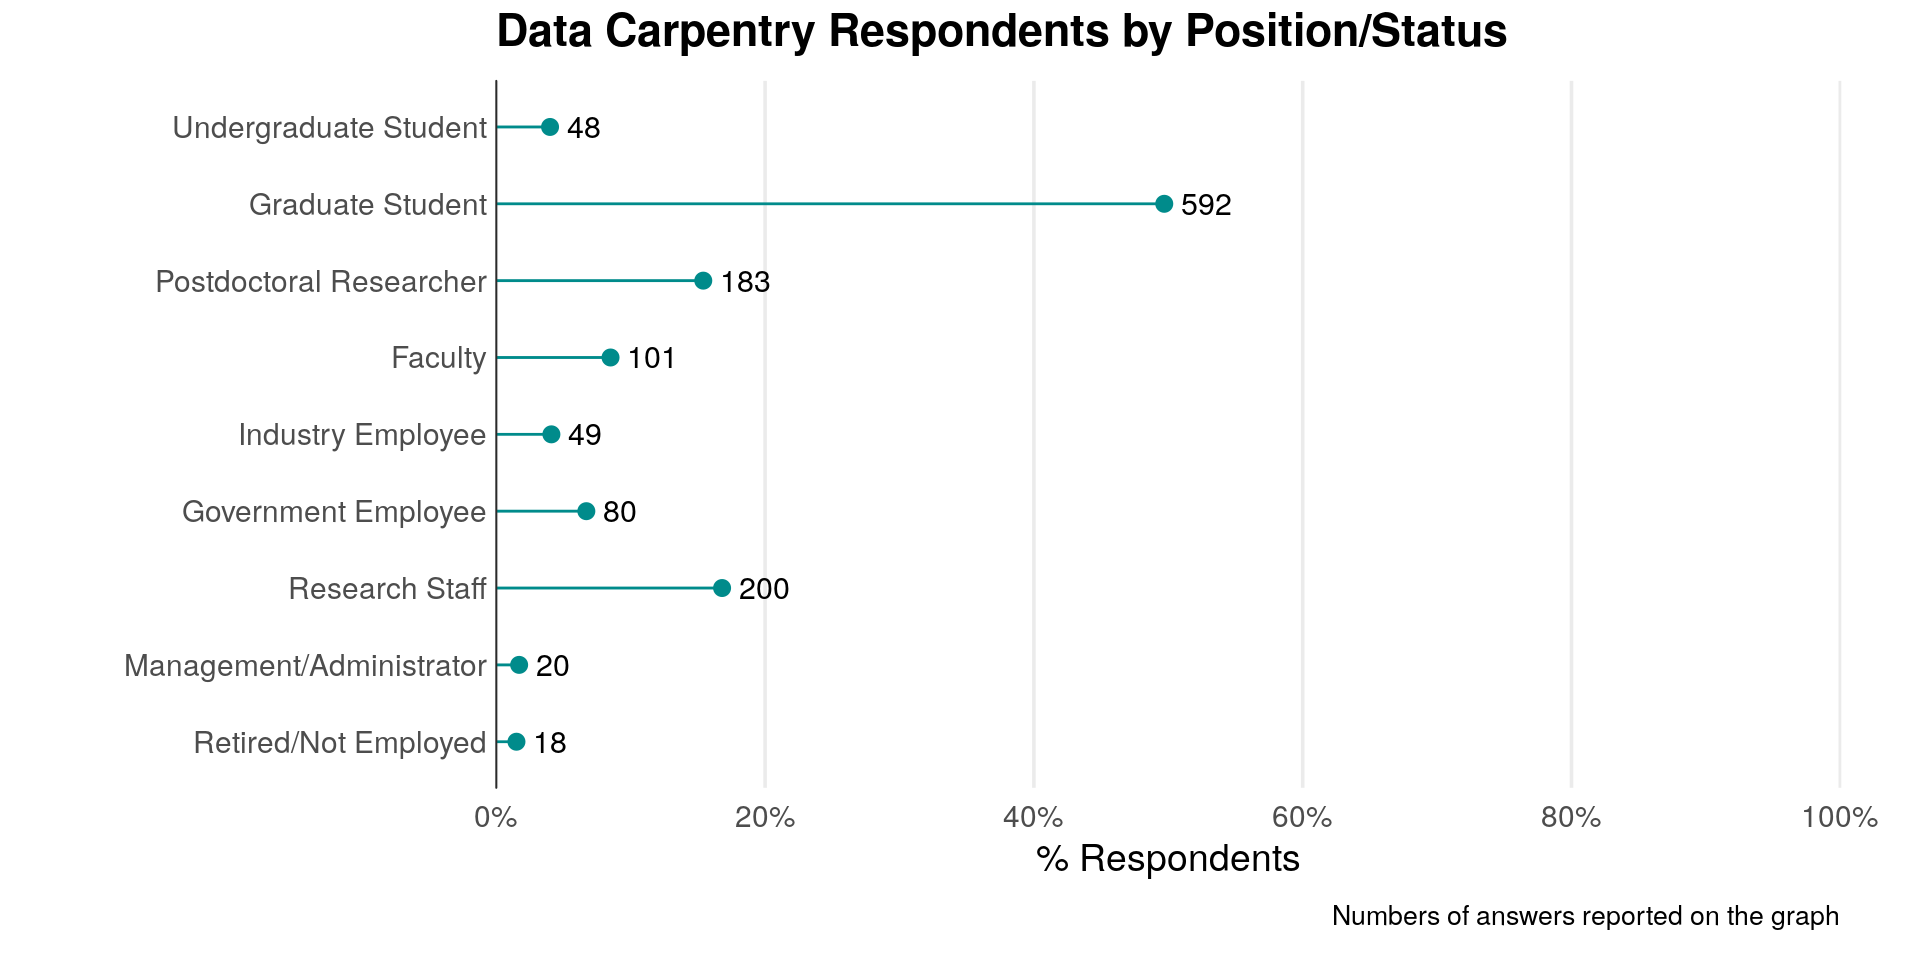
\includegraphics[width=\maxwidth]{../figures/dc-status-plot-1}

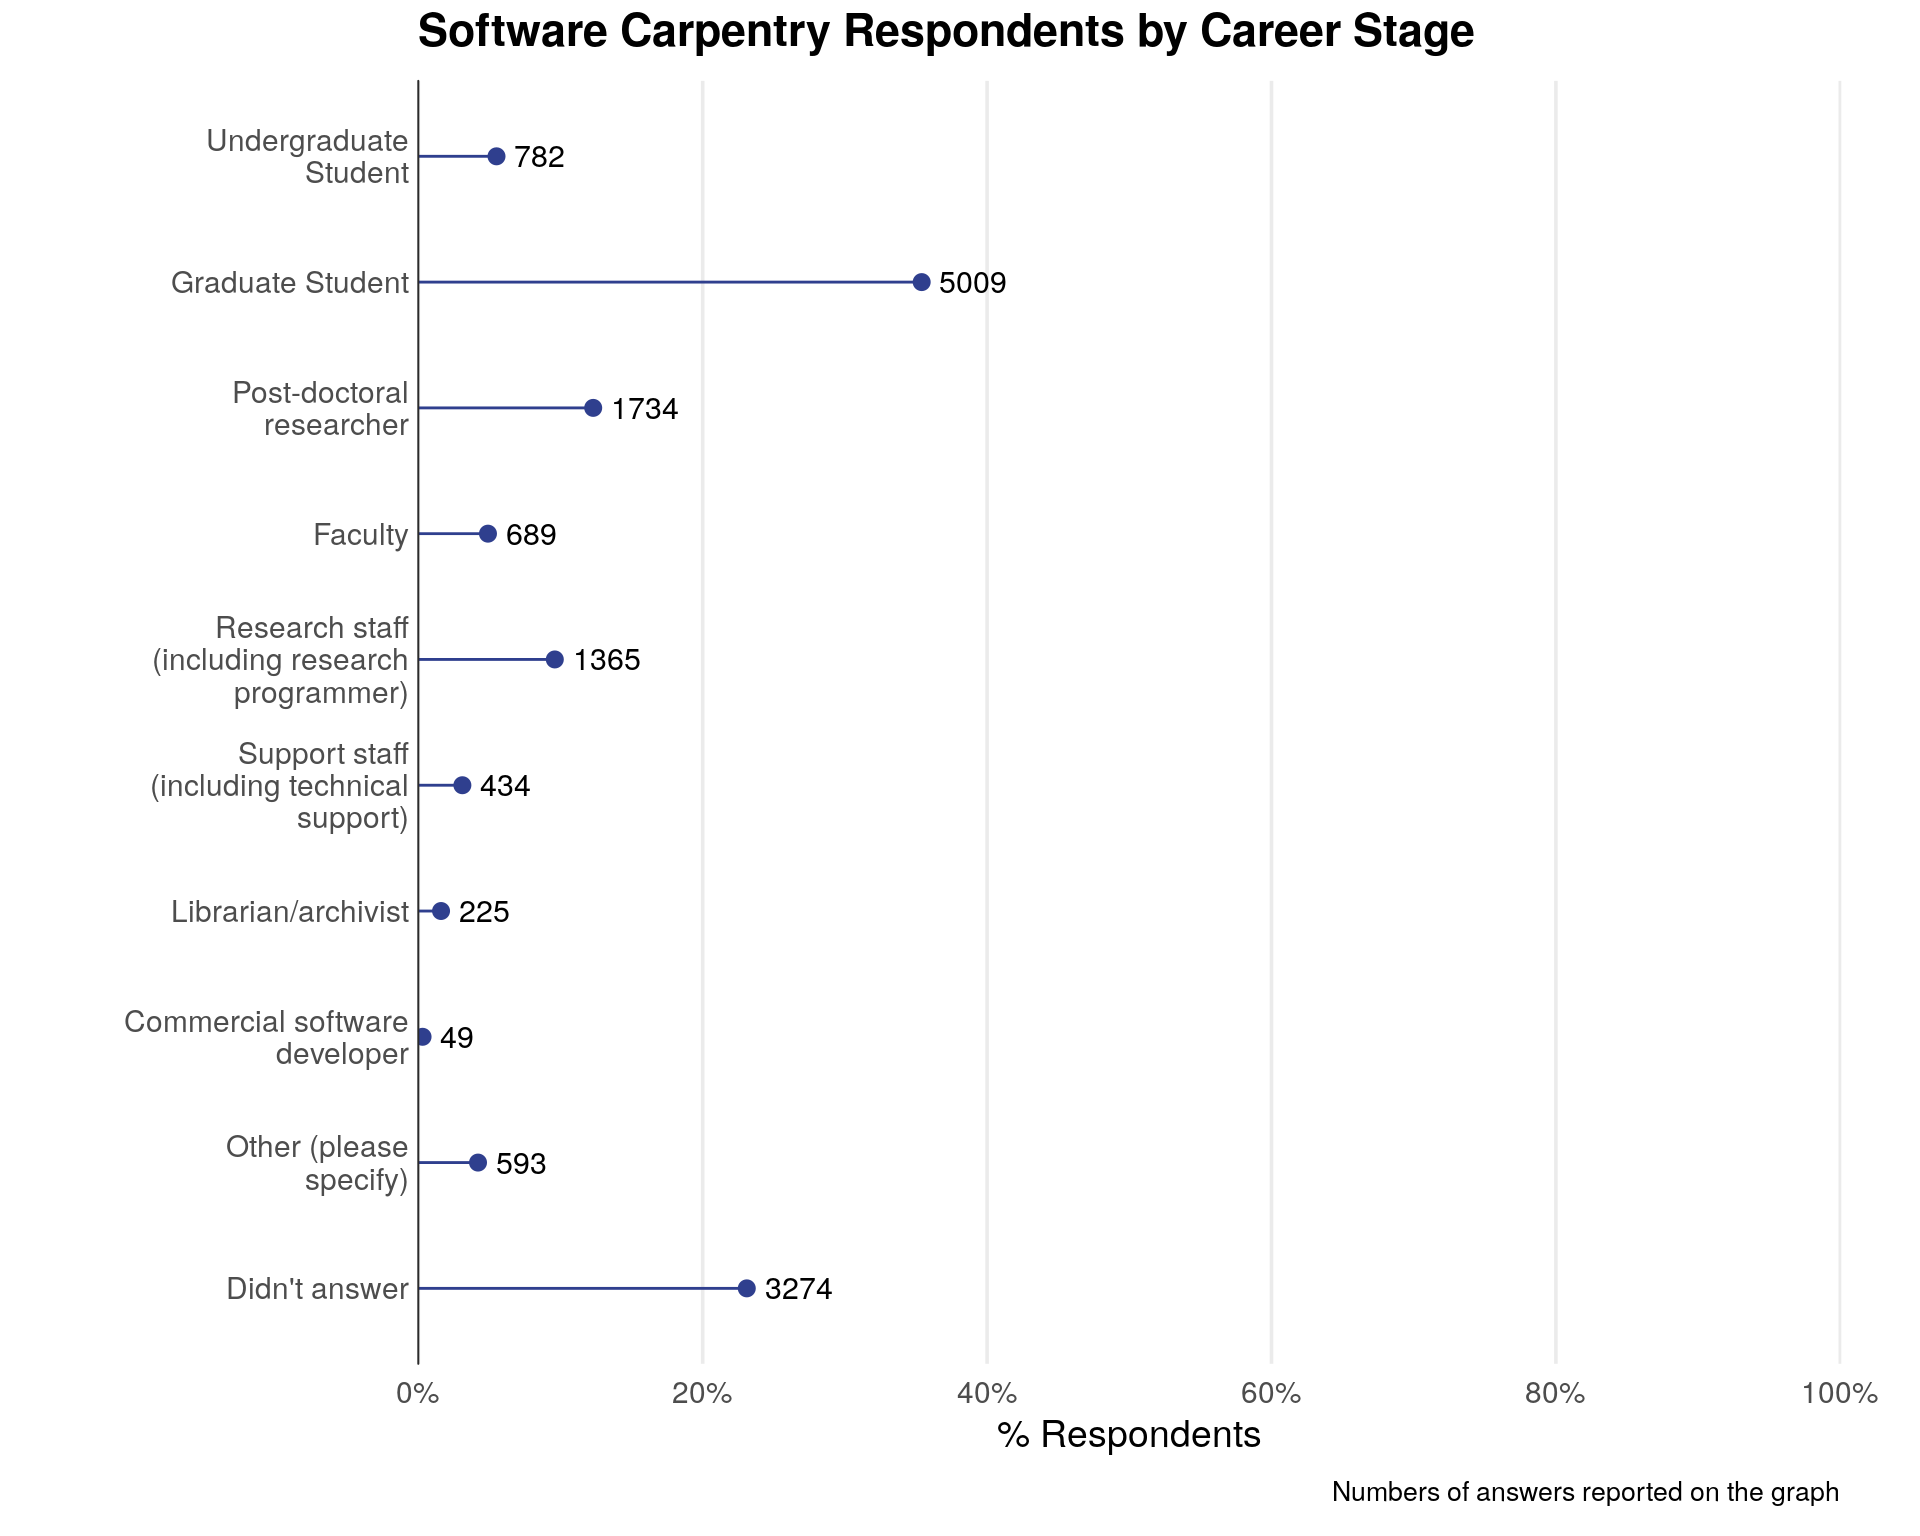
\includegraphics[width=\maxwidth]{../figures/swc-status-plot-1}

\subsubsection{Learners' operating
system}\label{learners-operating-system}

Gender and racial/ethnic identity information is collected for U.S.
participants, as we are keen to increase the number of diverse
instructors and learners we serve. This information is provided below
for the learners attending your workshops.

\begin{longtable}[]{@{}lrr@{}}
\toprule
Operating System Respondents Use in Data Carpentry Workshops & n &
\%\tabularnewline
\midrule
\endhead
Windows & 661 & 53.3\tabularnewline
Apple/Mac OS & 512 & 41.3\tabularnewline
UNIX/Linux & 50 & 4.0\tabularnewline
Not sure & 17 & 1.4\tabularnewline
\bottomrule
\end{longtable}

\subsubsection{Gender and Racial/Ethnic
Identity}\label{gender-and-racialethnic-identity}

\begin{longtable}[]{@{}lrr@{}}
\toprule
Data Carpentry's U.S. Respondents' Gender Identity & n &
\%\tabularnewline
\midrule
\endhead
Female & 322 & 56.6\tabularnewline
Male & 223 & 39.2\tabularnewline
Transgender female & 2 & 0.4\tabularnewline
Transgender male & 0 & 0.0\tabularnewline
Gender variant/non-conforming & 0 & 0.0\tabularnewline
Prefer not to answer & 8 & 1.4\tabularnewline
Didn't answer & 14 & 2.5\tabularnewline
\bottomrule
\end{longtable}

\begin{longtable}[]{@{}lrr@{}}
\toprule
Data Carpentry's U.S. Respondents Racial/Ethnic Identity & n &
\%\tabularnewline
\midrule
\endhead
American Indian or Alaska Native & 4 & 0.7\tabularnewline
Asian & 152 & 27.7\tabularnewline
Black or African American & 25 & 4.6\tabularnewline
Hispanic or Latino(a) & 57 & 10.4\tabularnewline
Native Hawaiian or Other Pacific Islander & 3 & 0.5\tabularnewline
White & 316 & 57.6\tabularnewline
I prefer not to say. & 28 & 5.1\tabularnewline
Other & 8 & 1.5\tabularnewline
\bottomrule
\end{longtable}

\begin{longtable}[]{@{}lrr@{}}
\toprule
Software Carpentry's U.S. Respondents' Gender Identity & n &
\%\tabularnewline
\midrule
\endhead
Female & 361 & 53.7\tabularnewline
Male & 305 & 45.4\tabularnewline
Other & 0 & 0.0\tabularnewline
Prefer not to say & 6 & 0.9\tabularnewline
\bottomrule
\end{longtable}

\begin{longtable}[]{@{}lrr@{}}
\toprule
Software Carpentry's U.S. Respondents' Racial/Ethnic Identity & n &
\%\tabularnewline
\midrule
\endhead
American Indian or Alaskan Native & 2 & 0.3\tabularnewline
Asian / Pacific Islander & 180 & 27.1\tabularnewline
Black or African American & 27 & 4.1\tabularnewline
Hispanic or Latino & 40 & 6.0\tabularnewline
Native Hawaiian or Other Pacific Islander & 1 & 0.2\tabularnewline
White / Caucasian & 344 & 51.7\tabularnewline
Multiple ethnicity / Other (please specify) & 29 & 4.4\tabularnewline
Prefer not to say & 42 & 6.3\tabularnewline
\bottomrule
\end{longtable}

\subsection{Summary}\label{summary}

This report focused on Data and Software Carpentry learners' skills,
perspectives, and experiences in your workshops. Our two-day coding
workshops increase researchers' daily programming usage, and confidence
in working with open source tools. If you'd like to discuss the results
from this report, please
\href{mailto:kariljordan@carpentries.org}{contact} Kari L. Jordan,
Director of Assessment and Community Equity for The Carpentries.


\end{document}
